
%%%%%%%%%%%%%%%%%%%%%%%%%%%%%%%%%%%%%%%%%%%%%%%%%%%%%%%%%%%%%%%%%%%%%%%%%%%%%%
\section{Advection and the finite-volume method}

\label{ch:adv:sndorder}

In these notes, we will typically use a {\em finite-volume} discretization.  Here we
explore this method for the
advection equation.  First we rewrite the advection equation in {\em
  conservation form}:
\begin{equation}
a_t + \left[f(a)\right]_x = 0
\label{eq:advect-cons}
\end{equation}
where $f(a) = ua$ is the flux of the quantity $a$.  In conservation form,
the time derivative of a quantity is related to the divergence of
its flux.

% figure created with figures/advection/fv-ghost.py
\begin{figure}[t]
\centering
\includegraphics[width=\linewidth]{fv_ghost}
\caption[A finite-volume grid with valid cells
  labeled]{\label{fig:fvghost} A finite-volume grid running from
  $\mathrm{lo}, \ldots, \mathrm{hi}$, with two ghost cells at each
  end.}
\end{figure}

Recall that in the finite-volume discretization, $\langle a\rangle_i$
represents the average of $a(x,t)$ over the interval $x_{i-\myhalf}$ to
$x_{i+\myhalf}$, where the half-integer indexes denote the zone edges
(i.e.\ $x_{i-\myhalf} = x_i - \Delta x/2$).  Figure~\ref{fig:fvghost}
shows an example of such a grid with 2 ghost cells at each end.  (For
simplicity of notation, we drop the $\langle \rangle$ going forward).
To discretize Eq.~\ref{eq:advect-cons}, we integrate it over a zone,
from ${x_{i-\myhalf}}$ to ${x_{i+\myhalf}}$, normalizing by the zone width,
$\Delta x$:
\begin{align}
\frac{1}{\Delta x} \int_{x_{i-\myhalf}}^{x_{i+\myhalf}} a_t \, dx &=
   - \frac{1}{\Delta x} \int_{x_{i-\myhalf}}^{x_{i+\myhalf}} \frac{\partial}{\partial x} f(a) \, dx \\
\frac{\partial}{\partial t} a_i &=
   - \frac{1}{\Delta x} \left \{ \left [f(a) \right ]_{i+\myhalf} - \left [f(a) \right ]_{i-\myhalf} \right \} \label{adv:eq:fvadv}
\end{align}
This is an evolution equation for the zone-average of $a$, and shows
that it updates in time based on the fluxes through the boundary of
the zone.

We now have a choice on how to proceed with the time-discretiation:
\begin{enumerate}
\item We can discretize ${\partial a_i}/{\partial t}$ directly as
  $(a_i^{n+1} - a_i^n)/\Delta t$.  Then to achieve second-order
  accuracy, we need to evaluate the righthand side of
  Eq.~\ref{adv:eq:fvadv} at the midpoint in time ($n+1/2$).  This
  gives rise to a predictor-corrector method (as described in
  \cite{colella:1990}.  Sometimes this is called a characteristic
  tracing method (a name which will be more clear when we discuss the
  Euler equations).

\item We can recognize that with the spatial discretization done, our
  PDE has now become an ODE, and we can use standard ODE methods (like
  Runge-Kutta) to integrate the system in time.  This is a method-of-lines
  integration.

\end{enumerate}

We'll look at both of these in the next sections.


\section{Second-order predictor-corrector scheme}

We discretize Eq.~\ref{adv:eq:fvadv} in time by evaluating the
righthand side at the midpoint in time---this gives a
centered-difference in time, which is second-order accurate:
\begin{equation}
\frac{a_i^{n+1} - a_i^n}{\Delta t} = -\frac{\left [f(a) \right ]_{i+\myhalf}^{n+\myhalf} - \left [f(a) \right ]_{i-\myhalf}^{n+\myhalf}}{\Delta x}
\label{eq:consupdate1d}
\end{equation}
To evaluate the fluxes at the half-time, we need the state at the
half-time, that is, we do :
\begin{equation}
\label{adv:eq:fluxeval}
\left [f(a) \right ]_{i+\myhalf}^{n+\myhalf} = f(a_{i+\myhalf}^{n+\myhalf}) \enskip .
\end{equation}
We construct a second-order accurate approximation to
$a_{i+\myhalf}^{n+\myhalf}$ by Taylor expanding the data in the cell
to the interface.  The construction of the interface state at the
midpoint in time is the prediction and the conservative update in the
correction here.

Notice that for each interface, there are two possible
interface states we can construct---one using the data to the left of
the interface (which we will denote with a ``L'' subscript) and the
other using the data to the right of the interface (denoted with an
``R'' subscript)---see Figure~\ref{fig:riemann_adv}.  These states are:
\begin{eqnarray}
a_{i+\myhalf,L}^{n+\myhalf} &=& a_i^n + \frac{\Delta x}{2} \left .\frac{\partial a}{\partial x} \right |_i + \frac{\Delta t}{2} \left .\frac{\partial a}{\partial t} \right |_i + \mathcal{O}(\Delta x^2) + \mathcal{O}(\Delta t^2) \nonumber \\
    &=& a_i^n + \frac{\Delta x}{2} \left .\frac{\partial a}{\partial x} \right |_i +  \frac{\Delta t}{2} \left ( - u \left .\frac{\partial a}{\partial x} \right |_i \right ) + \ldots \nonumber \\
    &=& a_i^n + \frac{\Delta x}{2} \left ( 1 - \frac{\Delta t}{\Delta x} u \right ) \left .\frac{\partial a}{\partial x} \right |_i +  \ldots \label{eq:statel}\\
%%
a_{i+\myhalf,R}^{n+\myhalf} &=& a_{i+1}^n - \frac{\Delta x}{2} \left .\frac{\partial a}{\partial x} \right |_{i+1} + \frac{\Delta t}{2} \left .\frac{\partial a}{\partial t} \right |_{i+1} + \mathcal{O}(\Delta x^2) + \mathcal{O}(\Delta t^2) \nonumber \\
    &=& a_{i+1}^n - \frac{\Delta x}{2} \left .\frac{\partial a}{\partial x} \right |_{i+1} +  \frac{\Delta t}{2} \left ( - u \left .\frac{\partial a}{\partial x} \right |_{i+1} \right ) + \ldots \nonumber \\
    &=& a_{i+1}^n - \frac{\Delta x}{2} \left ( 1 + \frac{\Delta t}{\Delta x} u \right ) \left .\frac{\partial a}{\partial x} \right |_{i+1} +  \ldots \label{eq:stater}
\end{eqnarray}
% figure created with figures/advection/riemann.py
\begin{figure}[t]
\centering
\includegraphics[width=5.0in]{riemann-adv}
\caption[The input state to the Riemann
  problem]{\label{fig:riemann_adv} The left and right interface state
  at the $i+\myhalf$ interface.  Here, the left state,
  $a_{i+\myhalf,L}^{n+\myhalf}$, was predicted to the interface from
  the zone to the left of the interface, using $a_i$, and the right
  state, $a_{i+\myhalf,R}^{n+\myhalf}$, was predicted to the interface
  from the zone to the right, using $a_{i+1}$.}
\end{figure}

A suitable estimate is needed for the slope of $a$ that appears in
these expressions (as $\partial a/\partial x$).  We can approximate
this simply as
\begin{equation}
\left . \frac{\partial a}{\partial x}\right |_i = \frac{a_{i+1} - a_{i-1}}{2 \Delta x} \label{eq:slopecentered}
\end{equation}
We can think of this method as reconstructing the function form of the
data from the cell-average data in each cell using a piecewise linear
polynomial.  Don't be worried that this looks like FTCS---we'll do
upwinding next.


We now have two states, $a_{i+\myhalf,L}^{n+\myhalf}$ and
$a_{i+\myhalf,R}^{n+\myhalf}$ separated by an interface---this is
called the {\em Riemann problem}.
%
The solution to this will depend on the equation being solved, and
results in a single state at the interface:
\begin{equation}
a_{i+\myhalf}^{n+\myhalf} = \mathcal{R}(a_{i+\myhalf,L}^{n+\myhalf},a_{i+\myhalf,R}^{n+\myhalf})
\end{equation}
In our case, the advection equation simply propagates the state to the
right (for $u > 0$), so the solution to the Riemann problem is to take
the left state (this is another example of upwinding).  That is we do:
\begin{equation}
\mathcal{R}(a_{i+\myhalf,L}^{n+\myhalf},a_{i+\myhalf,R}^{n+\myhalf}) = \left \{ \begin{array}{ccc} a_{i+\myhalf,L}^{n+\myhalf} & u > 0 \\[2mm] a_{i+\myhalf,R}^{n+\myhalf} & u < 0 \end{array} \right .
\label{eq:riemannsolve}
\end{equation}
To complete the update, we use this interface state to evaluate the
flux and update the advected quantity via Eq.~\ref{eq:consupdate1d}
and \ref{adv:eq:fluxeval}.

Boundary conditions are implemented by filling the ghost cells outside
each end of the domain based on data in the interior.  Note that at
the very left edge of the domain, the state
$a^{n+\myhalf}_{\mathrm{lo}-\myhalf}$ requires the construction of states on
the left and right.  The left state at that interface,
$a^{n+\myhalf}_{\mathrm{lo}-\myhalf,L}$ depends on the slope reconstructed in
the $\mathrm{lo}-1$ ghost cell, $\partial a/\partial x
|_{\mathrm{lo}-1}$.  This in turn is constructed using a limited
center-difference that will consider the value in the cell to the
left, $\mathrm{lo-2}$.  Therefore, we need two ghost cells at each end
of the domain for this method---figure~\ref{fig:advect_ghost}
illustrates this.  Higher-order limiters may require even more ghost
cells.

% figure from figures/advection/riemann_bc.py
\begin{figure}[t]
\centering
\includegraphics[width=\linewidth]{riemann-bc}
\caption[Reconstruction at the domain boundary]
        {\label{fig:advect_ghost} Reconstruction near the boundary,
          showing the need for two ghostcells.  Here we see the left
          and right state at the left physical boundary of the domain
          (marked as $\mathrm{lo}-\myhalf$).  The gray dotted lines
          are the piecewise constant cell averages and the red lines
          are the reconstructed slopes.  Note that we need the slope
          in $\mathrm{lo}-1$ to get the left interface state at
          $\mathrm{lo}-\myhalf$, and that slope in turn needed the
          data in zone $\mathrm{lo}-2$ to construct a
          centered-difference.}
\end{figure}


\begin{exercise}[A second-order finite-volume solver for linear advection]
{\label{adv:ex:fv} Write a second-order solver for the linear advection
  equation.  To mimic a real hydrodynamics code, your code should have
  routines for finding initializing the state, filling boundary conditions,
  computing the timestep,
  constructing the interface states, solving the Riemann problem, and
  doing the update.  The problem flow should look like:
  \begin{itemize}
    \item set initial conditions
    \item main evolution loop---loop until final time reached
    \begin{itemize}
      \item fill boundary conditions
      \item get timestep (Eq.~\ref{eq:timestep})
      \item compute interface states (Eqs.~\ref{eq:statel} and \ref{eq:stater})
      \item solve Riemann problem at all interfaces (Eq.~\ref{eq:riemannsolve})
      \item do conservative update (Eqs.~\ref{eq:consupdate1d} and \ref{adv:eq:fluxeval})
    \end{itemize}
  \end{itemize}
Use both the top-hat and Gaussian initial conditions and periodic boundary
conditions and compare to the first-order method.  See Figure~\ref{fig:fvadvect}.
}
\end{exercise}

\begin{figure}
\centering
% figure from codes/advection/fv_advection.py
\includegraphics[width=0.8\linewidth]{fv-advect}
\caption[Second-order finite-volume advection]
{\label{fig:fvadvect} Second-order finite volume advection showing the
result of advecting a tophat profile through five periods with both
unlimited and limited slopes.  This calculation used 64 zones and
$\cfl=0.7$. \\
\hydroexdoit{\href{https://github.com/zingale/hydro_examples/blob/master/advection/advection.py}{advection.py}}}
\end{figure}

\subsection{Limiting}

The second-order method likely showed some oscillations in the
solution, especially for the top-hat initial conditions.  {\em
  Godunov's theorem} says that any monotonic linear method for
advection is first-order accurate (see, e.g.,~\cite{laney}).  In this
context, monotonic means that no new minima or maxima are introduced.
The converse is true too, which suggests that in order to have a
second-order accurate method for this linear equation, the algorithm
itself must be nonlinear.

\begin{exercise}[Limiting and overshoots]
{To remove the oscillations in
practice, we limit the slopes to ensure that no new minima or maxima are
introduced during the advection process.  There are many choices for
limited slopes.  A popular one is the {\em minmod} limiter.  Here, we
construct the slopes in the interface states as:
\begin{equation}
\left . \frac{\partial a}{\partial x} \right |_i = \mathtt{minmod} \left (
  \frac{a_i - a_{i-1}}{\Delta x}, \frac{a_{i+1} - a_i}{\Delta x} \right )
\end{equation}
instead of Eq.~\ref{eq:slopecentered}.
with
\begin{equation}
\mathtt{minmod}(a,b) = \left \{
    \begin{array}{ll}
    a & \mathit{if~} |a| < |b| \mathrm{~and~} a\cdot b > 0 \\
    b & \mathit{if~} |b| < |a| \mathrm{~and~} a\cdot b > 0 \\
    0 & \mathit{otherwise}
    \end{array}
  \right .
\end{equation}
Use this slope in your second-order advection code and notice that the
oscillations go away---see Figure~\ref{fig:fvadvect}.}
\end{exercise}

We can get a feel for what happens with and without limiting
pictorially. \MarginPar{add a discussion on how a limiter is
  designed/constructed} Figures~\ref{fig:limitingex} and
\ref{fig:limitingexb} show the evolution of an initial discontinuity
with and without limiting.  Without limiting, we see an overshoot
behind the discontinuity and an undershoot ahead of it---these develop
after only a single step.  With each additional step, the overshoots
and undershoots move further away from the discontinuity.  In
contrast, the case with limiting shows no over- or undershoots around
the initial discontinuity.  By the end of the evolution, we see that
the profile is much narrower in the limiting case than in the case
without limiting.

See the text by LeVeque~\cite{leveque:2002} for alternate choices of
limiters. Note: most limiters will have some sort of test on the
product of a left-sided and right-sided difference ($a\cdot b$
above)---this is $< 0$ at an extremum, which is precisely where we
want to limit.

% these two sets of figures can be created with
% figures/advection/rea-limitex.py
\begin{figure}[h]
\centering
\includegraphics[width=0.75\linewidth]{rea-nolimit-start_001} \\
\includegraphics[width=0.75\linewidth]{rea-nolimit-start_002} \\
\includegraphics[width=0.75\linewidth]{rea-nolimit-start_003} \\
\includegraphics[width=0.75\linewidth]{rea-nolimit-start_004} \\
\includegraphics[width=0.75\linewidth]{rea-nolimit-start_005} \\
\includegraphics[width=0.75\linewidth]{rea-nolimit-start_006}
%\includegraphics[width=0.55\linewidth]{rea-nolimit-start_007} \\
%\includegraphics[width=0.55\linewidth]{rea-nolimit-start_008} \\
\caption[The effect of no limiting on initially discontinuous data]{\label{fig:limitingex}Initially discontinuous data evolved for several steps with
  no limiting.  Notice that there are overshoots and undershoots
  surrounding the discontinuity.}
\end{figure}

\begin{figure}[h]
\centering
\includegraphics[width=0.75\linewidth]{rea-start_001} \\
\includegraphics[width=0.75\linewidth]{rea-start_002} \\
\includegraphics[width=0.75\linewidth]{rea-start_003} \\
\includegraphics[width=0.75\linewidth]{rea-start_004} \\
\includegraphics[width=0.75\linewidth]{rea-start_005} \\
\includegraphics[width=0.75\linewidth]{rea-start_006}
%\includegraphics[width=0.55\linewidth]{rea-start_007}
%\includegraphics[width=0.55\linewidth]{rea-start_008} \\
\caption[The effect of limiters on initially discontinuous
  data]{\label{fig:limitingexb}Initially discontinuous data evolved
  for several steps with limiting.  Note that unlike the sequence
  without limiting (Figure~\ref{fig:limitingex}), the
  discontinuity remains sharper with limiting and there are no over-
  or undershoots.}
\end{figure}

A slightly more complex limiter is the MC limiter (monotonized central
difference).  First we define an extrema test,
\begin{equation}
\xi = (a_{i+1} - a_i) \cdot (a_i - a_{i-1})
\end{equation}
Then the limited difference is
\begin{equation}
\left . \frac{\partial a}{\partial x} \right |_i =
 \left \{
\begin{array}{ll}
\min \left [ \frac{| a_{i+1} - a_{i-1} |}{2 \Delta x},
              2 \frac{| a_{i+1} - a_i |}{\Delta x},
              2 \frac{| a_{i} - a_{i-1} |}{\Delta x}
      \right ]  \mathrm{sign}(a_{i+1} - a_{i-1}) &  \xi > 0 \\
0 & \mathit{otherwise}
\end{array}
\right .
\end{equation}
%
Note that a slightly different form of this limiter is presented in
\cite{leveque:2002}, where all quantities are in a {\tt minmod}, which appears to limit a bit less.
This is second-order accurate for smooth flows.

The main goal of a limiter is to reduce the slope near extrema.
Figure~\ref{fig:limit} shows a finite-volume grid with the original
data, cell-centered slopes, and MC limited slopes.  Note that near the
strong gradients is where the limiting kicks in.  The different limiters
are all constructed by enforcing a condition requiring the method to be
{\em total variation diminishing}, or TVD.  More details on TVD limiters
can be found in \cite{toro:1997,leveque:2002}.

% this figure can be create with figures/advection/generalgrid.py
\begin{figure}
\centering
\includegraphics[width=\linewidth]{generalgrid}
\caption[Piecewise linear slopes with an without
  limiting]{\label{fig:limit} A finite-volume grid showing the cell
  averages (gray, dotted, horizontal lines), unlimited center-difference slopes
  (gray, solid) and MC limited slopes (red).  Note that in zones $i$ and
  $i+1$, the slopes are limited slightly, so as not to overshoot or
  undershoot the neighboring cell value.  Cell $i-1$ is not limited at
  all, whereas cells $i-2$, and $i+2$ are fully limited---the slope is
  set to $0$---these are extrema.}
\end{figure}

A popular extension of the MC limiter is the $4^\mathrm{th}$-order MC
limiter, which is more accurate in smooth flows (this is shown in
\cite{colella:1985}, Eqs. 2.5 and 2.6; and \cite{colella:1990},
Eq. 191).

\begin{exercise}[Limiting and reduction in order-of-accuracy]
{Show analytically that if you fully limit the slopes
  (i.e.\ set $\partial a/\partial x |_i = 0$, that the second-order
  method reduces to precisely our first-order finite-difference discretization,
  Eq.~\ref{eq:fo}.  }
\end{exercise}

It is common to express the slope simply as the change in the state variable:
\begin{equation}
\Delta a_i = \left . \frac{\partial a}{\partial x} \right |_i \Delta x
\end{equation}
and to indicate the limited slope as $\overline{\Delta a}_i$.



%%%%%%%%%%%%%%%%%%%%%%%%%%%%%%%%%%%%%%%%%%%%%%%%%%%%%%%%%%%%%%%%%%%%%%%%%%%%%%
\subsection{Reconstruct-evolve-average}

Another way to think about these methods is as a reconstruction,
evolve, and average (R-E-A) process (see Figure~\ref{fig:rea}).

We can write the conservative update as:
\begin{align}
a_i^{n+1} &= a_i^n + \frac{\Delta t}{\Delta x}
    (u a^{n+\myhalf}_{i-\myhalf} - u a^{n+\myhalf}_{i+\myhalf} ) \\
          &= a_i^n + \cfl (a^{n+\myhalf}_{i-\myhalf} - a^{n+\myhalf}_{i+\myhalf} )
\end{align}
If we take $u > 0$, then the Riemann problem will always choose the
left state, so we can write this as:
\begin{equation}
a_i^{n+1} = a_i^n +
     \cfl \biggl [\underbrace{\left (a_{i-1}^n + \frac{1}{2} (1-\cfl) \Delta a_{i-1} \right )}_{a_{i-\myhalf,L}} -
              \underbrace{\left (a_{i}^n + \frac{1}{2} (1-\cfl) \Delta a_{i} \right )}_{a_{i+\myhalf,L}}
       \biggr ] \label{eq:rea_orig}
\end{equation}

If we instead look at this via the R-E-A procedure, we write the reconstructed
$a$ in each zone in the form of a piecewise linear polynomial
\begin{equation}
a_i(x) = a_i + \frac{\Delta a_i}{\Delta x} (x - x_i)
\end{equation}
Consider zone $i$.
If we are advecting with a CFL number $\cfl$, then that means that the fraction
$\cfl$ of the zone immediately to the left of the $i-\myhalf$ interface will advect
into zone $i$ over the timestep.  And only the fraction $1-\cfl$ in zone $i$
immediately to the right of the interface will stay in that zone.  This
is indicated by the shaded regions in Figure~\ref{fig:rea}.

The average of the quantity $a$ from zone $i-1$ that will advect into
zone $i$ is
\begin{eqnarray}
\mathcal{I}_< &=& \frac{1}{\cfl \Delta x}
   \int_{x_{i-\myhalf} - \cfl\Delta x}^{x_{i-\myhalf}} a_{i-1}(x) dx \\
%
 &=& \frac{1}{\cfl \Delta x}
   \int_{x_{i-\myhalf} - \cfl\Delta x}^{x_{i-\myhalf}}
        \left [ a_{i-1} + \frac{\Delta a_{i-1}}{\Delta x} (x - x_{i-1} ) \right ] dx  \\
 &=& a_{i-1} + \frac{1}{2} \Delta a_{i-1} (1-\cfl)
\end{eqnarray}

And the average of the quantity $a$ in zone $i$ that will remain in zone $i$
is
\begin{eqnarray}
\mathcal{I}_> &=& \frac{1}{(1-\cfl) \Delta x}
   \int_{x_{i-\myhalf}}^{x_{i-\myhalf} + (1-\cfl) \Delta x} a_{i}(x) dx \\
%
 &=& \frac{1}{(1-\cfl) \Delta x}
   \int_{x_{i-\myhalf}}^{x_{i-\myhalf} + (1-\cfl)\Delta x}
        \left [ a_{i} + \frac{\Delta a_{i}}{\Delta x} (x - x_{i} ) \right ] dx  \\
 &=& a_{i} - \frac{1}{2} \Delta a_{i} \cfl
\end{eqnarray}

The final part of the R-E-A procedure is to average the over the
advected profiles in the new cell.  The weighted average of the
amount brought in from the left of the interface and that that remains
in the cell is
\begin{align}
a_i^{n+1} &= \cfl \mathcal{I}_< + (1 - \cfl) \mathcal{I}_>  \\
          &= \cfl \left [ a^n_{i-1} + \frac{1}{2} \Delta a_{i-1} (1 - \cfl) \right ]
   + (1-\cfl) \left [ a^n_i - \frac{1}{2} \Delta a_i \cfl \right ] \\
          &= a^n_i + \cfl \left [a^n_{i-1} + \frac{1}{2}(1 - \cfl) \Delta a_{i-1} \right ]
           - \cfl \left [ a^n_i + \frac{1}{2} (1-\cfl) \Delta a_i \right ]
\end{align}
This is identical to Eq.~\ref{eq:rea_orig}.  This demonstrates that the
R-E-A procedure is equivalent to our reconstruction, prediction of the
interface states, solving the Riemann problem, and doing the
conservative flux update.

% this figure sequence is created by figures/advection/rea.py
\begin{figure}
\centering
\includegraphics[width=\linewidth]{rea-start} \\
\includegraphics[width=\linewidth]{rea-reconstruction} \\
\includegraphics[width=\linewidth]{rea-trace} \\
\includegraphics[width=\linewidth]{rea-evolve} \\
\includegraphics[width=\linewidth]{rea-final}
\caption[The Reconstruct-Evolve-Average procedure]{\label{fig:rea}
  Reconstruct-Evolve-Average.  The top panel shows the original
  cell-average data.  The second panel shows the (limited) piecewise
  linear reconstruction of the data.  Assuming a CFL number of 0.6 and
  advection to the right, the shaded regions in the third panel show
  the data that will wind up in cell $i$ after advecting for a single
  step.  The fourth panel shows the piecewise-linear data advected to
  the right by 0.6 of a cell-width (corresponding to a CFL of 0.6).
  The final panel shows the new averages of the data, constructed by
  averaging the advected piecewise linear data in each cell.}
\end{figure}


\begin{exercise}[Convergence testing]
{ Run the first-order solver for several different values of $\Delta x$,
each a factor of 2 smaller than the previous.  Compute $\epsilon$ for
each resolution and observe that it converges in a first-order fashion
(i.e.\ $\epsilon$ decreases by 2 when we decrease $\Delta x$ by a factor of 2).

\noindent Do the same with the second-order solver and observe that it
converges as second-order. However: you may find less than
second-order if your initial conditions have discontinuities and you
are limiting.  Figure~\ref{fig:advnorm} shows the convergence of the
method with no limiting, MC, and minmod limiting, $\cfl = 0.8$, and a
Gaussian initial condition for 5 periods.}
\end{exercise}

% figure from hydro_examples: advection/advection.py
\begin{figure}[t]
\centering
\includegraphics[width=0.8\linewidth]{plm-converge}
\caption[Convergence of second-order finite-volume advection]
        {\label{fig:advnorm} Convergence for the second-order
          finite-volume method with no limiting, MC, and minmod limiting advecting a
          Gaussian initial profile with $\cfl = 0.8$ for 5 periods. \\
        \hydroexdoit{\href{https://github.com/zingale/hydro_examples/blob/master/advection/advection.py}{advection.py}}}
\end{figure}

\begin{figure}[ht]
\centering
\includegraphics[width=0.8\linewidth]{fv-gaussian-limiters} \\[1em]
\includegraphics[width=0.8\linewidth]{fv-tophat-limiters}
\caption[Effect of different limiters on evolution]
        {\label{fig:limiter_panel} The effect of different limiters on the
          evolution of a Gaussian initial profile (top) and a tophat initial
          profile (bottom), using $\cfl = 0.8$ and 5 periods. \\
        \hydroexdoit{\href{https://github.com/zingale/hydro_examples/blob/master/advection/advection.py}{advection.py}}}
\end{figure}

As seen in figure~\ref{fig:advnorm}, the choice of limiters can have a great
effect on the accuracy.  Figure~\ref{fig:limiter_panel} shows the Gaussian and
tophat profiles with several different limiters.

\section{Method of lines approach}
\label{adv:sec:mol_2d}

In the above constructions, we computed a time-centered flux by
predicting the interface state to the half-time (by Taylor-expanding
in time through $\Delta t /2$).  Instead, we can recognize that with
the spatial discretization done in Eq.~\ref{eq:adv:fvadv}, we are left
with an ordinary differential equation in time that can then be solved
using standard ODE techniques.

Substituting in the flux as $f(a) = ua$, we have the ODE:
\begin{equation}
\ddt{a_i} = - \frac{u a_{i+1/2} - u a_{i-1/2}}{\Delta x}
\end{equation}
Note that there is no time-level indicated on the righthand side.  We
find the interface values of $a$ by interpolating in space only.  For
a second-order accurate method, we can use a piecewise linear
reconstruction (see Figure~\ref{fig:advection:riemann-mol}), and
evaluate the interface states as simply the point on the reconstructed
line on the interface, e.g.,
\begin{align}
a_{i+\myhalf,L} &= a_{i} + \frac{1}{2} \Delta a_{i} \\
a_{i+\myhalf,R} &= a_{i+1} - \frac{1}{2} \Delta a_{i+1}
\end{align}
%
\begin{figure}[t]
\centering
\includegraphics[width=\linewidth]{riemann-mol}
\caption[Method-of-lines spatial
  reconstruction]{\label{fig:advection:riemann-mol} Piecewise linear
  reconstruction of the zones showing the interface states used with
  the method of lines approach.}
\end{figure}
%
The same limiting ideas discussed above apply here.  As usual, we
resolve the left-right degeneracy on the interface by solving the
Riemann problem:
\begin{equation}
a_{i+\myhalf,j} = \mathcal{R}(a_{i+\myhalf,j,L}, a_{i+\myhalf,j,R})
\end{equation}
Once we have this interface state, we can integrate the ODE.  A
Runge-Kutta method works fine here (it should be atleast second-order
to match the spatial accuracy).
\section{Multi-dimensional advection}

The two-dimensional linear advection equation is:
\begin{equation}
a_t + u a_x + v a_y = 0
\label{eq:advect2d}
\end{equation}
where $u$ is the velocity in the $x$-direction and $v$ is the velocity in
the $y$-direction.  We denote the average of $a(x,y,t)$ in a zone $i,j$ as
$a_{i,j}$.  Here, $i$ is the index in the $x$-direction and $j$ is the
index in the $y$-direction.  A 2-d grid is shown in Figure~\ref{fig:2dgrid}.
Just as in the one-dimensional case, we will extend the domain with a
perimeter of ghost cells to set the boundary conditions.

% this is create by figures/advection/2dgrid.py
\begin{figure}[h]
\centering
\includegraphics[width=4.0in]{2dgrid}
\caption[A 2-d grid with zone-centered indexes]{\label{fig:2dgrid} A
  simple 2-d grid with the zone-centered indexes.  The $\times$s mark
  the left and right interface states at the upper edge of the $i,j$ zone in each
  coordinate direction.  For a finite-volume discretization, $a_{i,j}$
  represents the average of $a(x,y)$ over the zone.}
\end{figure}

To derive the finite-volume form of the update, we start by writing
this in conservative form.  Since $u$ and $v$ are constant, we can
move them inside the divergences:
\begin{equation}
a_t + (u a)_x + (v a)_y = 0
\label{eq:advect2d-cons}
\end{equation}
This is the form we will integrate over zones.  As before, we will
define the average of $a$ in a zone by integrating it over the
volume:
\begin{equation}
a_{i,j} = \frac{1}{\Delta x \Delta y}
   \int_{x_{i-\myhalf}}^{x_{i+\myhalf}} \int_{y_{j-\myhalf}}^{y_{j+\myhalf}}
   a(x,y,t) \, dx \, dy
\end{equation}
Integrating Eq.~\ref{eq:advect2d-cons} over $x$ and $y$, we have:
\begin{align}
\frac{1}{\Delta x \Delta y}
  \int_{x_{i-\myhalf}}^{x_{i+\myhalf}}
  \int_{y_{j-\myhalf}}^{y_{j+\myhalf}} a_t \, dx \, dy =
  &- \frac{1}{\Delta x \Delta y}
       \int_{x_{i-\myhalf}}^{x_{i+\myhalf}} \int_{y_{j-\myhalf}}^{y_{j+\myhalf}}
      (u a)_x \, dx \, dy \nonumber \\
  &- \frac{1}{\Delta x \Delta y}
       \int_{x_{i-\myhalf}}^{x_{i+\myhalf}} \int_{y_{j-\myhalf}}^{y_{j+\myhalf}}
      (v a)_y \, dx \, dy
\end{align}
or using the divergence theorem,
\begin{align}
\label{eq:adv:multiddivergence}
 \frac{\partial a_{i,j}}{\partial t} =
  &- \frac{1}{\Delta x\Delta y} \int_{y_{j-\myhalf}}^{y_{j+\myhalf}}
     \left \{ (u a)_{i+\myhalf,j} - (u a)_{i-\myhalf,j} \right \} dy \nonumber \\
  &- \frac{1}{\Delta x\Delta y} \int_{x_{i-\myhalf}}^{x_{i+\myhalf}}
     \left \{ (v a)_{i,j+\myhalf} - (v a)_{i,j-\myhalf} \right \} dx
\end{align}

Now we integrate over time---the left side of our expression becomes
just the difference between the new and old state.
\begin{align}
 a_{i,j}^{n+1} - a_{i,j}^n =
  &- \frac{1}{\Delta x\Delta y} \int_{t^n}^{t^{n+1}} \int_{y_{j-\myhalf}}^{y_{j+\myhalf}}
     \left \{ (u a)_{i+\myhalf,j} - (u a)_{i-\myhalf,j} \right \} dy dt \nonumber \\
  &- \frac{1}{\Delta x\Delta y} \int_{t^n}^{t^{n+1}} \int_{x_{i-\myhalf}}^{x_{i+\myhalf}}
     \left \{ (v a)_{i,j+\myhalf} - (v a)_{i,j-\myhalf} \right \} dx dt
\label{eq:update2du}
\end{align}
We define the flux through the interface as the average over the face
of that interface and time: \MarginPar{is there a way to illustrate this, as some space-time diagram?}
\begin{itemize}
\item x-face:
\begin{equation}
\langle (ua)_{i+\myhalf,j}\rangle_{(t)} = \frac{1}{\Delta y \Delta t}
    \int_{t^n}^{t^{n+1}} \int_{y_{j-\myhalf}}^{y_{j+\myhalf}} (ua)_{i+\myhalf,j}\, dy dt
\end{equation}
\item y-face
\begin{equation}
\langle (va)_{i,j+\myhalf}\rangle_{(t)} = \frac{1}{\Delta x \Delta t}
    \int_{t^n}^{t^{n+1}} \int_{x_{i-\myhalf}}^{x_{i+\myhalf}} (va)_{i,j+\myhalf}\, dx dt
\end{equation}
\end{itemize}
where $\langle . \rangle_{(t)}$ denotes the time-average over the face.
For a second-order accurate method in time, we replace the average in
time with the flux at the midpoint in time and the average over the face
with the flux at the center of the face:
\begin{equation}
\langle (ua)_{i+\myhalf,j} \rangle_{(t)} \approx (ua)_{i+\myhalf,j}^{n+\myhalf}
\end{equation}
Then we have:
\begin{equation}
a_{i,j}^{n+1} = a_{i,j}^n - \Delta t \left [
   \frac{(ua)_{i+\myhalf,j}^{n+\myhalf} - (ua)_{i-\myhalf,j}^{n+\myhalf}}{\Delta x} +
   \frac{(va)_{i,j+\myhalf}^{n+\myhalf} - (va)_{i,j-\myhalf}^{n+\myhalf}}{\Delta y} \right ]
\end{equation}

For the advection problem, since $u$ and $v$ are constant, we need
to find the interface states of $a$ alone.
There are two methods for computing these interface states,
$a_{i\pm\myhalf,j}^{n+\myhalf}$ on $x$-interfaces and  $a_{i,j\pm\myhalf}^{n+\myhalf}$ on $y$-interfaces:
dimensionally split and unsplit.  Dimensionally split methods are
easier to code, since each dimension is operated on independent of the
others, so you can simply call a one-dimensional method for each
direction.  Unsplit methods, however, are more accurate and less
susceptible to grid effects.  \MarginPar{show an example + refs? Zalesak test?}

\subsection{Dimensionally split}
\label{adv:sec:dimensionalsplit}

In a split method, we update the state in each coordinate direction
independently.  This is simple and a straightforward way to use
one-dimensional methods in multi-d.  To be second-order accurate in
time, we do {\em Strang splitting}~\cite{strang}, where we alternate
the order of the dimensional updates each timestep.  An update through
$\Delta t$ consists of $x$ and $y$ sweeps and appears as:
\begin{eqnarray}
 \frac{a_{i,j}^\star - a_{i,j}^n}{\Delta t} &=&
  - \frac{ u a_{i+\myhalf,j}^{n+\myhalf} - u a_{i-\myhalf,j}^{n+\myhalf} }{\Delta x} \label{eq:splitx}\\
 \frac{a_{i,j}^{n+1} - a_{i,j}^\star}{\Delta t} &=&
  - \frac{ v a_{i,j+\myhalf}^{\star,n+\myhalf} - v a_{i,j-\myhalf}^{\star,n+\myhalf} }{\Delta y} \label{eq:splity}
\end{eqnarray}
Here, Eq.~\ref{eq:splitx} is the update in the $x$-direction.  In
constructing the interface states, $a_{i+\myhalf,j}^{n+\myhalf}$ and
$a_{i-\myhalf,j}^{n+\myhalf}$, we do the exact same procedure as the
one-dimensional case, constructing the left and right states at each
interface and then solving the same Riemann problem to find the unique
state on the interface.  Each dimensional sweep is done without
knowledge of the other dimensions.  For example, in the $x$-update, we
are solving:
\begin{equation}
a_t + u a_x = 0
\label{eq:advect1dx}
\end{equation}
and in the $y$-update, we are solving:
\begin{equation}
a_t + v a_y = 0
\end{equation}

The construction of the interface states largely mimics the one-dimensional
case (Eq.~\ref{eq:statel} and \ref{eq:stater}).  For example, the
$a_{i+\myhalf,j,L}^{n+\myhalf}$ state is:
\begin{eqnarray}
a_{i+\myhalf,j,L}^{n+\myhalf} &=& a_{i,j}^n +
  \frac{\Delta x}{2} \left .\frac{\partial a}{\partial x} \right |_{i,j} +
  \frac{\Delta t}{2} \left .\frac{\partial a}{\partial t} \right |_{i,j} +
  \mathcal{O}(\Delta x^2) + \mathcal{O}(\Delta t^2) \nonumber \\
 &=& a_{i,j}^n +
   \frac{\Delta x}{2} \left .\frac{\partial a}{\partial x} \right |_{i,j} +
   \frac{\Delta t}{2} \left (
   - u \left .\frac{\partial a}{\partial x} \right |_{i,j} \right
   ) + \ldots \nonumber \\
    &=& a_{i,j}^n +
   \frac{\Delta x}{2} \left ( 1 - \frac{\Delta t}{\Delta x} u \right )
   \left .\frac{\partial a}{\partial x} \right |_{i,j} +
   \ldots \label{eq:statels}
\end{eqnarray}
Notice that when substituting for $\partial a / \partial t$, we use
the one-dimensional split version of the advection equation
(Eq.~\ref{eq:advect1dx}) instead of the full multi-dimensional
equation.  There are no $y$-direction terms that come into play in the
split method when considering the $x$-direction.

The $x$-update
(Eq.~\ref{eq:splitx}) updates the state only accounting for the
$x$-fluxes---we denote this intermediate state with the `$\star$'
superscript.  For the $y$-update, we construct our interface states in
the analogous way as in the $x$-direction, but begin with the `$\star$'
state instead of the old-time state.  In this fashion, the $y$-update
`sees' the result of the $x$-update and couples things together.

To achieve second-order accuracy in time, it is necessary to alternate
the directions of the sweeps each timestep, i.e., $x$-$y$ then $y$-$x$.
Furthermore, this pair of sweeps should use the same timestep, $\Delta t$.


\subsection{Unsplit multi-dimensional advection}
\label{adv:sec:unsplit_2d}

The unsplit case differs from the dimensionally split case in two
ways: (1) in predicting the interface states, we use knowledge of the
flow in the transverse direction, and (2), only a single conservative
update is done per timestep, with all directions updating
simultaneously.  See \cite{colella:1990} for more details.  This idea
is sometimes called the ``corner transport upwind'' or CTU method.

The construction of the $a_{i+\myhalf,j,L}^{n+\myhalf}$ interface state appears as
\begin{eqnarray}
a_{i+\myhalf,j,L}^{n+\myhalf} &=& a_{i,j}^n +
  \frac{\Delta x}{2} \left .\frac{\partial a}{\partial x} \right |_{i,j} +
  \frac{\Delta t}{2} \left .\frac{\partial a}{\partial t} \right |_{i,j} +
  \mathcal{O}(\Delta x^2) + \mathcal{O}(\Delta t^2) \nonumber \\
 &=& a_{i,j}^n +
   \frac{\Delta x}{2} \left .\frac{\partial a}{\partial x} \right |_{i,j} +
   \frac{\Delta t}{2} \left (
   - u \left .\frac{\partial a}{\partial x} \right |_{i,j}
   - v \left .\frac{\partial a}{\partial y} \right |_{i,j} \right
   ) + \ldots \nonumber \\
    &=& \underbrace{a_{i,j}^n +
   \frac{\Delta x}{2} \left ( 1 - \frac{\Delta t}{\Delta x} u \right )
   \left .\frac{\partial a}{\partial x} \right |_{i,j}}_{\hat{a}_{i+\myhalf,j,L}^{n+\myhalf}} \underbrace{-
   \frac{\Delta t}{2} v \left .\frac{\partial a}{\partial y} \right |_{i,j}}_{\mathrm{``transverse~flux~difference''}} +
   \ldots \label{eq:statelu}
\end{eqnarray}
The main difference between the split and unsplit interface states is the
explicitly appearance of the ``transverse flux difference'' in the unsplit
interface state.  We rewrite this as:
\begin{equation}
a_{i+\myhalf,j,L}^{n+\myhalf} = \hat{a}_{i+\myhalf,j,L}^{n+\myhalf}
   - \frac{\Delta t}{2} v \left .\frac{\partial a}{\partial y} \right |_{i,j}
\end{equation}
Here, the $\hat{a}_{i+\myhalf,j,L}^{n+\myhalf}$ term is just the normal
prediction without considering the transverse direction (e.g., Eq.~\ref{eq:statels}).  The basic
update procedure is:
\begin{itemize}
\item Construct the normal predictor term, $\hat{a}_{i+\myhalf,j,L}^{n+\myhalf}$,
in a fashion identical to the one-dimensional and split methods.  We
compute these one-dimensional $\hat{a}$'s at the left and right every
interface in both coordinate directions.  Note that these states are
still one-dimensional, since we have not used any information from the
transverse direction in their computation.

\item Solve a Riemann problem at each of these interfaces:
\begin{eqnarray}
a^T_{i+\myhalf,j} &=& \mathcal{R}(\hat{a}_{i+\myhalf,j,L}^{n+\myhalf},
                              \hat{a}_{i+\myhalf,j,R}^{n+\myhalf}) \\
a^T_{i,j+\myhalf} &=& \mathcal{R}(\hat{a}_{i,j+\myhalf,L}^{n+\myhalf},
                              \hat{a}_{i,j+\myhalf,R}^{n+\myhalf}) \\
\end{eqnarray}
These states are given the `$^T$' superscript since they are the states
that are used in computing the transverse flux difference.

\item Correct the
previously computed normal interface states (the $\hat{a}$'s) with
the transverse flux difference:
\begin{equation}
a_{i+\myhalf,j,L}^{n+\myhalf} = \hat{a}_{i+\myhalf,j,L}^{n+\myhalf}
   - \frac{\Delta t}{2} v \frac{a^T_{i,j+\myhalf} - a^T_{i,j-\myhalf}}{\Delta y}
\end{equation}
Notice that the
fluxes that are differenced for the left state are those that are
transverse, but to the left of the interface.  Similarly, for the
right state, it would be those that are transverse, but to the right
of the interface:
\begin{equation}
a_{i+\myhalf,j,R}^{n+\myhalf} = \hat{a}_{i+\myhalf,j,R}^{n+\myhalf}
   - \frac{\Delta t}{2} v \frac{a^T_{i+1,j+\myhalf} - a^T_{i+1,j-\myhalf}}{\Delta y}
\end{equation}
\end{itemize}
A similar procedure happens at the $y$-interfaces.

Figure~\ref{fig:unsplitstates} illustrates the steps involved in
the construction of the $a_{i+\myhalf,j,L}^{n+\myhalf}$ state.  \MarginPar{more panels illustrating the sequence?}
%
% this is created by figures/advection/2dgrid-hat.py
% and                                  2dgrid-transverse.py
\begin{figure}
\centering
\includegraphics[width=0.7\linewidth]{2dgrid-hat} \\
\includegraphics[width=0.7\linewidth]{2dgrid-transverse}
\caption[The construction of an interface state with the transverse
  component]{\label{fig:unsplitstates} The construction of the
  $a_{i+\myhalf,j,L}^{n+\myhalf}$ state.  Top: first we compute the
  $\hat{a}$'s---here we show all of the $\hat{a}$'s that will be used
  in computing the full left interface state at $(i+\myhalf,j)$.  Bottom:
  after the transverse Riemann solves, we have the two transverse
  states ($a^T_{i,j+\myhalf}$ and $a^T_{i,j-\myhalf}$) that will be
  differenced and used to correct $\hat{a}_{i+\myhalf,j,L}^{n+\myhalf}$
  (illustrated by the dotted lines) to make $a_{i+\myhalf,j,L}^{n+\myhalf}$.}
\end{figure}

Once all of the full states (normal prediction $+$ transverse flux
difference) are computed to the left and right of all the interfaces
($x$ and $y$), we solve another Riemann problem to find the final
state on each interface.
\begin{equation}
a_{i+\myhalf,j}^{n+\myhalf} = \mathcal{R}(a_{i+\myhalf,j,L}^{n+\myhalf},
                                  a_{i+\myhalf,j,R}^{n+\myhalf}) \\
\end{equation}
The final conservative update is then done via Eq.~\ref{eq:update2du}.

See \cite{colella:1990} for more details on this unsplit method,
and \cite{saltzman:1994} for details of the extension to 3-d.

Figures~\ref{fig:adv:gaussian-2d} and \ref{fig:adv:tophat-2d} show the
advection of a smooth Gaussian and a discontinuous tophat diagonally on
a coarse $32\times 32$ zone domain.  Each show a diffusion of the
initial function, similar to what we saw in 1-d.  In the tophat, we
also see a slight undershoot on the trailing side of the tophat after
one period.




% run as: ./pyro.py advection smooth inputs.smooth
% visualized as: ./plot.py -W 7.7 -H 6 -o smooth_init.pdf advection smooth_0000
\begin{figure}
\centering
\includegraphics[width=0.48\linewidth]{smooth_init}\hspace{1em}
\includegraphics[width=0.48\linewidth]{smooth_final}
\caption[Advection of Gaussian profile in 2-d]
  {\label{fig:adv:gaussian-2d} Advection of a Gaussian profile
  with $u = v = 1$ for one period on a $32\times 32$ grid, with $\cfl =
  0.8$.  This was run with \pyro\ as {\tt ./pyro.py advection smooth
    inputs.smooth}}
\end{figure}

\begin{figure}
\centering
\includegraphics[width=0.48\linewidth]{tophat_init}\hspace{1em}
\includegraphics[width=0.48\linewidth]{tophat_final}
\caption[Advection of tophat profile in 2-d]{\label{fig:adv:tophat-2d} Advection of a tophat function with
  $u = v = 1$ for one period on a $32\times 32$ grid, with $\cfl = 0.8$.
  This was run as {\tt ./pyro.py advection tophat inputs.tophat}}
\end{figure}


\subsection{Timestep limiter for multi-dimensions}
\label{sec:adv:timestep}

The timestep criterion we used in one-dimension
(Eq.~\ref{eq:timestep}) needs to be generalized for multi-dimensions.
For the dimensionally split case, since we are basically piecing
together two one-dimensional sweeps, the timestep limit is usually taken
as:
\begin{equation}
\label{eq:adv:timestep:multid}
\Delta t = \cfl \min \left \{ \frac{\Delta x}{|u|} , \frac{\Delta y}{|v|} \right \}
\end{equation}
This is, for example, the construction that is used with the
dimensionally-split hydrodynamics solver in the original Flash
code~\cite{flash}\footnote{although, the paper does not explicitly
  write this out}.  \MarginPar{does the prometheus MPA 449 write it out?}
Stability requires picking a CFL number, $\cfl \le 1$.

A general extension of the timestep restriction for a
fully-multi-dimensional algorithm is often written in the form (see,
e.g., \cite{shuosher:1989b})
\begin{equation}
\label{eq:adv:timstep:mol}
\Delta t = \cfl \left ( \sum_{i=1}^d \frac{|\Ub \cdot \mathbf{e}_d|}{\Delta x_d} \right )^{-1}
\end{equation}
where $d$ is the coordinate direction, $\Ub = (u, v)$ is the velocity
vector, and $\mathbf{e}_d$ is the unit vector in direction $d$.  For
these methods $\cfl \lesssim 1$.  This is usually more restrictive than
Eq.~\ref{eq:adv:timestep:multid}.

For the CTU method described above, \cite{colella:1990} argues that
the inclusion of the transverse information removes some of the some
of the instability inherent in simpler schemes, allowing for a larger
timestep, restricted by Eq.~\ref{eq:adv:timestep:multid}.

Note, because of the different form of the timestep limiters here, it
is not enough to simply cite a CFL number when describing results, you
must also explain which form of the timestep calculation
(Eq.~\ref{eq:adv:timestep:multid} or Eq.~\ref{eq:adv:timstep:mol}) is
being used.

\subsection{Method-of-lines in multi-dimensions}

The multidimensional version of method-of-lines integration
follows the ideas from the one-dimensional case.
We can start with Eq.~\ref{eq:adv:multiddivergence}, and define
the fluxes over though a face as:
\begin{itemize}
\item x-face:
\begin{equation}
\langle (ua)_{i+\myhalf,j} \rangle = \frac{1}{\Delta y}
    \int_{y_{j-\myhalf}}^{y_{j+\myhalf}} (ua)_{i+\myhalf,j}\, dy
\end{equation}
\item y-face
\begin{equation}
\langle (va)_{i,j+\myhalf} \rangle = \frac{1}{\Delta x}
    \int_{x_{i-\myhalf}}^{x_{i+\myhalf}} (va)_{i,j+\myhalf}\, dx
\end{equation}
\end{itemize}
These are similar to the expressions above, except there is no
integral over time.  Again, to second order in space, we can just
use the flux evaluated at the midpoint in the face:
\begin{equation}
\langle (ua)_{i+\myhalf,j} \rangle \approx (ua)_{i+\myhalf,j}
\end{equation}
The result is the ODE:
\begin{equation}
\frac{d a_{i,j}}{d t} =
   - \frac{(ua)_{i+\myhalf,j} - (ua)_{i-\myhalf,j}}{\Delta x}
   - \frac{(va)_{i,j+\myhalf} - (va)_{i,j-\myhalf}}{\Delta y}
\end{equation}

For the interface states, we separately construct slopes in each
dimension: $\Delta^{(x)}a_{i,j}$ is the slope in the $x$-direction,
and $\Delta^{(y)}a_{i,j}$ is the slope in the $y$-direction.  Then
the interface states are:
\begin{align}
a_{i+\myhalf,j,L} &= a_{i,j} + \frac{1}{2} \Delta a^{(x)}_{i,j} \\
a_{i+\myhalf,j,R} &= a_{i+1,j} - \frac{1}{2} \Delta a^{(x)}_{i+1,j}
\end{align}
and
\begin{align}
a_{i,j+\myhalf,L} &= a_{i,j} + \frac{1}{2} \Delta a^{(y)}_{i,j} \\
a_{i,j+\myhalf,R} &= a_{i,j+1} - \frac{1}{2} \Delta a^{(y)}_{i,j+1}
\end{align}

With these interface states, we have the method for evaluating the
righthand side of our ODE.  We can then evolve the ODE using a
Runge-Kutta integration method.  At each stage of the RK integration,
we do the same construction of the interface states, solve the Riemann
problem, etc.  Notice that unlike the directionally-split method, we
are doing the update in both directions at the same time---we are
relying on the ODE integrator to do the coupling in the different
directions for us.

This construction is a lot simpler than the unsplit method described
previously.  The cost of this simplicity is a reduced range of
stability.

Performaing the stability analysis here is much more complicated.  For
simplicity, consider a simple first-order upwind scheme in
two-dimensions.  Higher order time integrators (like RK4) will have
separate stages that look like a first-order-in-time update, so this
stability analysis can be thought of as applying to a single stage.
Our difference equation is:
\begin{equation}
\frac{a^{n+1}_{i,j} - a^n_{i,j}}{\Delta t} = - u \frac{a^n_{i,j} - a^n_{i-1,j}}{\Delta x}
- v \frac{a^n_{i,j} - a^n_{i,j-1}}{\Delta y}
\end{equation}
We introduce a single-mode Fourier function, as before, but this time
with a mode in each direction:
\begin{equation}
a^n_{i,j} = A^n e^{Ii\theta}e^{Ij\phi}
\end{equation}
Next, to simplify things, we'll assume that $u = v$, and $\Delta x = \Delta y$,
then $\cfl = u \Delta t/ \Delta x = v \Delta t / \Delta y$.
Inserting this into our difference equation gives:
\begin{equation}
\frac{A^{n+1}}{A^n} = 1 - \cfl \left (1 - e^{-I\theta} \right ) - \cfl \left (1 - e^{-I\phi} \right )
\end{equation}
This form looks very close to the one-dimensional case, but it is
difficult to analytically find the values of $\cfl$, but we can
numerically find the maximum $ | {A^{n+1}}/{A^n} |^2$ for $\theta \in
[0, 2\pi]$ and $\phi \in [0, 2\pi]$ as a function of $\cfl$.  In doing
this, we find that this discretization is unstable ($| {A^{n+1}}/{A^n}
|^2 > 1$) for $\cfl > 1/2$\footnote{See the script
  \href{https://github.com/zingale/hydro_examples/blob/master/compressible/cfl.py}{cfl.py}}.

This restriction is $1/d$, where $d$ is the dimensionality, and it is
analogous to the difference between the timestep limits for stability
from the more generous Eq.~\ref{eq:adv:timestep:multid} to the more
restrictive Eq.~\ref{eq:adv:timstep:mol}.
This reduced $\cfl$ for stability is discussed in
\cite{shuosher:1989b} (see section 4), and is also discussed in
\cite{titarevtoro,mccorquodalecolella}.  Different reconstruction and
integration methods can vary this limit some, for instance, the fourth-order
method in \cite{mccorquodalecolella} allows for $\Delta t \sum_{i=1}^d (|\Ub \cdot \mathbf{e}_d|)/\Delta x_d  \lesssim 1.4$.  Total variation diminishing Runge-Kutta methods are popular
for this application~\cite{gottliebshu:1996}.

% run as:
%   ./pyro.py advection_rk tophat inputs.tophat
%   ./plot.py -W 7.7 -H 6 -o tophat_rk4_cfl08.pdf advection_rk tophat_0040
%
%   ./pyro.py advection_rk tophat inputs.tophat driver.cfl=0.4
%   ./plot.py -W 7.7 -H 6 -o tophat_rk4_cfl04.pdf advection_rk tophat_0080
\begin{figure}
\centering
\includegraphics[width=0.48\linewidth]{tophat_rk4_cfl08}\hspace{1em}
\includegraphics[width=0.48\linewidth]{tophat_rk4_cfl04}
\caption[Advection of tophat function with method-of-lines integration]
  {\label{fig:adv:tophat-2d-rk4} Advection of a tophat function using
  the method-of-lines approach with 4th-order Runge-Kutta time integration.
  We use $u = v = 1$ for one period on a $32\times 32$ grid.  On the left
  is $\cfl = 0.8$---this is clearly unstable.  On the right is $\cfl = 0.4$,
  which is stable.
  This was run as {\tt ./pyro.py advection\_rk tophat inputs.tophat}}
\end{figure}



\section{High-Order Finite difference methods}
\label{sec:ho-fd}

Chapter~\ref{ch:advection} introduced numerical methods for the linear
advection equation
\begin{equation}
\label{eq:ho-advect}
a_t + u a_x = 0
\end{equation}
that were first or second order in space. The advantages of using numerical
methods that are higher order can be large, especially when in regions where
the flow is smooth. However, these must be balanced against the additional
computational cost and complexity. In addition, many higher order methods do no
better than second order methods in cases with discontinuities.

\subsection{The problem with higher-order finite volume methods}

The finite volume approach outlined in chapter~\ref{ch:fv}
%\todo{label missing in fv tex file?}
matches the physics of hyperbolic balance
laws perfectly, by maintaining the conservation of appropriate quantities using
the fluxes through the surfaces of each control volume or computational cell.
However, this leads to significant computational costs and complexities when
going beyond second order methods.

The inter-cell fluxes are computed by integrals over the face of the
computational cell. In one dimension the face is a single point and the
integral needs the flux evaluated at a single point, as in
equation~\ref{eq:consup}. In higher dimensions the face is one dimensional
(e.g., a line) or two dimensional (e.g., a square) and so the integral must be
approximated by evaluating the flux at \emph{multiple} points. If we use Gauss
quadrature, this means that a third order method would require at least two
flux evaluations per face in two dimensions, and typically four evaluations per
face in three dimensions.

%
% This comment about the timestep doesn't hold in general, as pointed out by
% Mike. I think it *is* relevant for directionally split codes where the
% transverse Riemann Problem isn't solved. That's probably too technical a
% distinction to make this early.
%
%As well as the additional computational cost, there is also typically an
%additional restriction on the timestep. Intuitively this can be seen by
%thinking about the flux evaluations again. We fix the values either side of the
%cell boundary in order to compute the flux at one point.  The timestep
%restriction is given by the time it take for information to propagate from a
%different flux evaluation point, which would change the information available.
%As we need to compute the flux at more points within the cell faces, the
%distance between points where the flux is evaluated goes down, reducing the
%time it takes for information to propagate from one point to another.

\subsection{Finite differences}

The conservative finite difference method starts from the endpoint for finite
volume methods, by considering the update formula~\eqref{eq:consup}
%\todo{is this the right equation to ref? Don't think it's labelled?}
\begin{equation}
\tag{\ref{eq:consup}}
\frac{\partial \langle \Uc\rangle_{i}}{\partial t} =
  - \frac{1}{\Delta x} \left \{ \Fb_{i+\myhalf} -
                                \Fb_{i-\myhalf} \right \}.
\end{equation}
In the finite difference method a interpretation used is different. We are now
thinking of
\begin{equation}
  \label{eq:fd-deriv}
  \frac{1}{\Delta x} \left \{ \Fb_{i+\myhalf} -
                                \Fb_{i-\myhalf} \right \}
\end{equation}
as representing a direct approximation to the derivative of the flux at $x_i$.
In particular, we are \emph{not} thinking of $\Fb_{i+\myhalf}$ as being
directly linked to the flux. Crucially the update still ensures global
conservation, as the ``flux'' term is re-used for neighbouring points in the
same way as in the finite volume case.

When we combine this viewpoint with the Method of Lines approach in
section~\ref{adv:sec:mol_2d}, the implementation of a high-order finite boils
down to
\begin{itemize}
  \item using a high-order time integration scheme (such as a high order
  Runge-Kutta method);
  \item finding a way that the finite difference in equation~\eqref{eq:fd-deriv}
  approximates the derivative of the flux both stably, and to a sufficiently
  high order.
\end{itemize}

\subsection{WENO reconstruction}
\label{sec:WENO}

\begin{figure}
  \includegraphics[width=0.96\linewidth]{weno-convergence}
  \caption[Convergence rate of high-order reconstructions]{A smooth sine function is reconstructed on the unit interval from the (integral-average) data, at the blue circles in the top plot, to the right, at the red triangles in the top plot. The convergence rate with grid resolution for the 5 point stencil of equation~\eqref{eq:weno-advection-5pt} and the 3 point stencils of equation~\eqref{eq:weno-advection-3pt} are shown to match expectations in the bottom plots. The error from the WENO reconstruction described in section~\ref{sec:WENO-algorithm} is, on this smooth function, converging with the expected order but larger in magnitude.}
  \label{fig:weno-convergence}
\end{figure}

For the advection equation with constant advection speed $u$, our higher-order
method requires us to find a high-order approximation to $a_{i+\myhalf}$. If we
considered the five points $a_{j}, j \in [i-2, \dots, i+2]$ then we could use
the information from all five of these points to approximate $a_{i+\myhalf}$ as
\begin{equation}
  \label{eq:weno-advection-5pt}
  a^{(\text{Fifth})}_{i+\myhalf} = \tfrac{1}{60} \left( 2 \langle a \rangle_{i-2} - 13 \langle a \rangle_{i-1} + 47 \langle a \rangle_{i} + 27 \langle a \rangle_{i+1} - 3 \langle a \rangle_{i+2} \right) + {\cal O}(\Delta x^5).
\end{equation}
Alternatively we could use only three of the points, in three different ways:
\begin{subequations}
  \label{eq:weno-advection-3pt}
  \begin{align}
    a^{(\text{Third}, 2)}_{i+\myhalf} &= \tfrac{1}{6} \left( 2 \langle a \rangle_{i-2} - 7 \langle a \rangle_{i-1} + 11 \langle a \rangle_{i} \right) + {\cal O}(\Delta x^3), \\
    a^{(\text{Third}, 1)}_{i+\myhalf} &= \tfrac{1}{6} \left( - \langle a \rangle_{i-1} + 5 \langle a \rangle_{i} + 2 \langle a \rangle_{i+1} \right) + {\cal O}(\Delta x^3), \\
    a^{(\text{Third}, 0)}_{i+\myhalf} &= \tfrac{1}{6} \left( 2 \langle a \rangle_{i} + 5 \langle a \rangle_{i+1} - \langle a \rangle_{i+2} \right) + {\cal O}(\Delta x^3).
  \end{align}
\end{subequations}

Which is better? The five point stencil gives higher order accuracy, but
includes information from both sides of the point. This ignores information from
the characteristics and, near discontinuities, will lead to Gibbs oscillations.
The three point stencils give lower accuracy. However, they give us the
flexibility to choose a stencil to avoid discontinuities, possibly using the
characteristic information. The advantages of the higher-order methods are illustrated by reconstructing a smooth function in figure~\ref{fig:weno-convergence}. The disadvantages of using a fixed stencil are illustrated by reconstructing a non-smooth function in figure~\ref{fig:weno-weights}.


\begin{exercise}[ENO stencils]
{Check that equations~\eqref{eq:weno-advection-5pt} and
\eqref{eq:weno-advection-3pt} give the claimed order of accuracy results.}
\end{exercise}

The method of choosing the ``best'' stencil (to avoid discontinuities as far as
possible) is called \emph{Essentially Non-Oscillatory} (ENO) reconstruction. It
is not as accurate as it could be given the size of the stencil it uses, and
the logical branches required to find the ``best'' stencil can reduce
computational performance.

An alternative that avoids the problems of ENO schemes are the \emph{Weighted}
ENO, or WENO, schemes. These use a combination of the possible ENO stencils to
reconstruct $a_{i+\myhalf}$. This relies on the observation that there are
constants $C_k$ such that, for example,
\begin{equation}
  \label{eq:WENO-C-weights}
  a^{(\text{Fifth})}_{i+\myhalf} = \sum_{k=0}^{2} C_k a^{(\text{Third}, r)}_{i+\myhalf}.
\end{equation}

\begin{exercise}[WENO weights]
{Check that the constants $C_0 = \tfrac{3}{10}, C_1 = \tfrac{3}{5}, C_2 =
\tfrac{1}{10}$ make equation~\eqref{eq:WENO-C-weights} consistent with
equations~\eqref{eq:weno-advection-5pt} and \eqref{eq:weno-advection-3pt}.}
\end{exercise}

The WENO methods work by retaining the sum over all stencils as in
equation~\eqref{eq:WENO-C-weights}, but adjusting the weights to avoid
oscillations. Ideally, in regions where the $a^{(0,1)}$ stencils include a
shock but the $a^{(2)}$ stencil does not the weights should be $\tilde{C}_0 = 0
= \tilde{C}_1$ and $\tilde{C}_2 = 1$. In order for this sum to make sense we
will need the weights to add to $1$.

\subsubsection{WENO algorithm}
\label{sec:WENO-algorithm}

\begin{figure}
  \includegraphics[width=0.96\linewidth]{weno-weights}
  \caption[WENO reconstruction and weights]{A non-smooth function is reconstructed on the unit interval. The 5 point stencil of equation~\eqref{eq:weno-advection-5pt} and the 3 point stencils of equation~\eqref{eq:weno-advection-3pt} both show oscillations near the discontinuity, whilst the WENO reconstruction does not. The WENO algorithm depends on measuring the smoothness of the function. The Jiang-Shu smoothness indicators $\beta$ are mostly zero, but spike near the discontinuity. This feeds into the weight $\omega$ that the WENO algorithm gives to each 3 point stencil it uses. Away from the discontinuity the weights revert to the optimal $C$ weights, but near the discontinuity a single $\omega$ weight dominates meaning only a single 3 point stencil is used.}
  \label{fig:weno-weights}
\end{figure}

We can now write out the full WENO algorithm of order $(2 r - 1)$. The constant
$r$ sets the size of the individual stencils as well as the (optimal) order of
the scheme. This section mostly uses the notation of Gerolymos et al.~\cite{Gerolymos2009}, and we will drop the integral average notation (so $\langle a \rangle_i$ will be denoted $a_i$).

First compute the individual stencils
\begin{equation}
  \label{eq:weno-stencils}
  a_{r, k, i+\myhalf} = \sum_{\ell=0}^{r-1} A_{r, k, \ell} a_{i+k-\ell}, \quad k = 0, \dots, r-1.
\end{equation}
Here the $A_{r, k, \ell}$ terms are constants which, for given scheme accuracy
$r$ are needed to compute the $k^{\text{th}}$ stencil.

We then want to combine these individual stencils to compute the WENO result.
For this we write
\begin{equation}
  \label{eq:weno-reconstruction}
  a_{r, WENO, i+\myhalf} = \sum_{k=0}^{r-1} \omega_{r, k, i+\myhalf} a_{r, k, i+\myhalf}.
\end{equation}
Here the $\omega_{r, k, i+\myhalf}$ terms are the weights that vary from point
to point. They must sum to one, so that we have a convex combination of the
stencils:
\begin{equation}
  \label{eq:weno-convex}
  \sum_{k=1}^{r-1} \omega_{r, k, i+\myhalf} = 1.
\end{equation}
We also want the weights to match the \emph{optimal} weights $C_{r, k}$ in
smooth regions. The optimal weights are defined such that
\begin{equation}
  \label{eq:weno-optimal}
  a_{r, WENO, i+\myhalf} = \sum_{k=0}^{r-1} C_{r, k} a_{r, k, i+\myhalf}
\end{equation}
is accurate to order ${\cal O}(\Delta x^{(2 r - 1)})$ when $q$ is smooth.

The \emph{choice} of how to get from the optimal weights $C_{r, k}$ to the
nonlinear weights $\omega_{r, k, i+\myhalf}$ defines the WENO scheme. The
standard choice of Jiang and Shu is to introduce a measure of the smoothness of
the $k^{\text{th}}$ stencil by computing the sum of the integral averages of
its derivatives from order $1$ up to order $2 r - 1$. For practical
implementation purposes this means computing the \emph{smoothness indicators}
$\beta_{r, k, i+\myhalf}$ as
\begin{equation}
  \label{eq:weno-smoothness}
  \beta_{r, k, i+\myhalf} = \sigma_{r, k, \ell, m} a_{i+k-\ell} a_{i+k-m}.
\end{equation}
The terms $\sigma_{r, k, \ell, m}$ are pre-computed constants which give the
coefficients in the quadratic form for the $k^{\text{th}}$ stencil of width $r$
in the reconstruction. These smoothness indicators are non-negative, and will
be large when the derivatives are large in magnitude. The Jiang and Shu weights
are then set by
\begin{subequations}
  \label{eq:weno-nonlinear-weights}
  \begin{align}
    \label{eq:weno-nonlinear-weights-omega}
    \omega_{r, k, i+\myhalf} &= \frac{\alpha_{r, k, i+\myhalf}}{\sum_{k=0}^{r-1} \alpha_{r, k, i+\myhalf}}, \\
      \label{eq:weno-nonlinear-weights-alpha}
    \alpha_{r, k, i+\myhalf} &= \frac{C_{r, k}}{\epsilon + \beta_{r, k, i+\myhalf}^2}.
  \end{align}
\end{subequations}
Here $\epsilon$ is a small number introduced to avoid division-by-zero problems.
The form of $\omega_{r, k, i+\myhalf}$ in
equation~\eqref{eq:weno-nonlinear-weights-omega} guarantees that the convex sum
condition in equation~\eqref{eq:weno-convex} holds. The form of $\alpha_{r, k,
i+\myhalf}$ ensures that when all the smoothness indicators $\beta_{r, k,
i+\myhalf}$ are the same magnitude the weights $\omega_{r, k, i+\myhalf}$ will
match the optimal weights $C_{r, k}$, but when a smoothness indicator is large
(i.e., when the associated stencil has large derivatives, typically associated
with discontinuities), the contribution of its associated stencil will be small.
An example of this is shown in figure~\ref{fig:weno-weights}.

Finally, we note that this method has reconstructed $a_{i+\myhalf}$ from the
left. For the advection equation case where the advection speed $u$ is positive
this is all we need: the characteristic information tells us that we should use
this reconstruction. In the case where the advection speed is negative we
should reconstruct from the right. In the implementation it is easiest to
implement only one reconstruction direction and pass the data in in reverse
order.


\begin{exercise}[WENO reconstruction]
{Taking the values for the $C$, $A$ and $\sigma$ constants from Gerolymos et
al.\ or Shu's review~\cite{Shu1997}, construct a WENO reconstruction method for
$r=2$. Check your results on smooth and non-smooth functions.}
\end{exercise}

\subsubsection{Implementation issues with WENO schemes}
\label{sec:weno-implementation}

A convergence test on the WENO schemes with $r=3$ and $r=5$ is shown in
figure~\ref{fig:weno-converge-gaussian-rk4}. This should be compared to
figure~\ref{fig:advnorm}, as in both a Gaussian profile is advected five
times around a periodic domain. The WENO schemes show higher absolute accuracy
for moderate size grids ($N \gtrsim 100$) and show faster convergence.

However, it is clear that whilst the $r=3$ method converges at fifth order as
expected, the $r=5$ WENO method does not converge at ninth order but at fourth
order. This is explained by the time integrator. We remember that any solver
has an error both from the spatial and the time discretization. In
figure~\ref{fig:weno-converge-gaussian-rk4} the time integrator is the classic
fourth order Runge-Kutta, and it is the error from this integrator that is
dominating.

To confirm this, figure~\ref{fig:weno-converge-gaussian} uses the eigth order
Dormand-Price Runge-Kutta method with adaptive step size control (using the
\texttt{scipy.integrate.ode} routine). Here we see high order convergence for
all $r$, and in each case the convergence rate is $2 r - 2$ for \textbf{no
reason I can understand}.

\begin{figure}[t]
\centering
% figure generated by hydro_examples/advection/weno.py
\includegraphics[width=0.8\linewidth]{weno-converge-gaussian-rk4}
\caption[High order WENO convergence rates for linear advection]
{\label{fig:weno-converge-gaussian-rk4} WENO solutions for advecting a Gaussian five periods, using two different orders. A fourth order Runge-Kutta method is used for time evolution. For $r=3$ we see the expected fifth ($2 r - 1$) order convergence. For $r=5$ we see fourth order, rather than the expected ninth order, convergence. This is as the error from the time integrator dominates. \\
\hydroexdoit{\href{https://github.com/zingale/hydro_examples/blob/master/advection/weno.py}{weno.py}}}
\end{figure}
%

\begin{figure}[t]
\centering
% figure generated by hydro_examples/advection/weno.py
\includegraphics[width=0.8\linewidth]{weno-converge-gaussian}
\caption[Very high order WENO convergence rates for linear advection]
{\label{fig:weno-converge-gaussian} WENO solutions for advecting a Gaussian one periods, using four different orders. An eighth order Dormand-Price Runge-Kutta method is used for time evolution. This minimizes the time integrator error and we see convergence at order $2 r - 2$ for all schemes, although the time integrator error eventually shows in the highest order case. \\
\hydroexdoit{\href{https://github.com/zingale/hydro_examples/blob/master/advection/weno.py}{weno.py}}}
\end{figure}
%

\subsection{Discontinuous Galerkin methods}
\label{sec:dg}

In addition to the issues with higher order schemes noted above, there is one
wasteful step that is worth noting. Each time a higher order scheme reconstructs
the data it constructs a high-order piecewise polynomial representation of the
data everywhere. Then, in the time update, most of this information is thrown
away. At the beginning of each timestep we only know the value of the function
(for finite difference approaches) or its integral average (for finite volume
approaches).

Some alternative methods store the \emph{moments} or \emph{modes} of the
solution, and update all of them. In these methods all of the information
needed to evaluate the solution is available at all times and locations, and
all the information is updated at every step. This should make the methods more
efficient and more local (with a smaller stencil, and hence better on parallel
machines). Their disadvantages will come in the timestep and with discontinuous
data.

The presentation here closely follows~\cite{hesthaven2018numerical} -- check
there for considerably more details, particularly on the theoretical results.

\subsubsection{Function basis and weak form}
\label{sec:dg_basis}

Recall that in this chapter we are looking at the advection equation
%
\begin{equation}
  \tag{\ref{eq:ho-advect}}
  a_t + u a_x = 0.
\end{equation}
%
We want to be able to compute the value of the function $a(t, x)$ at any point.
We can do this by writing $a$ in terms of a \emph{function basis} $\psi_n(t, x)$
as
%
\begin{equation}
  \label{eq:dg_fn_basis}
  a(t, x) = \sum_n \hat{a}_n \psi_n(t, x).
\end{equation}
%
Here the \emph{modes} or \emph{modal coefficients} $\hat{a}_n$ are constants. An
example of a function basis would be
%
\begin{equation}
  \label{eq:dg_monomial_basis}
  \begin{aligned}
    \psi_{0}(t, x) &= 1, & \psi_{1}(t, x) &= x, & \psi_{2}(t, x) &= t, \\
    \psi_{3}(t, x) &= \tfrac{1}{2} x^2, & \psi_{4}(t, x) &= \tfrac{1}{2} t^2, &
    \psi_{5}(t, x) &= x t.
  \end{aligned}
\end{equation}
%
These six modes will perfectly describe any function that remains quadratic for
all space and time.

It is often more convenient the explicitly separate space and time, as we saw
using the Method of Lines in section~\ref{adv:sec:mol_2d}. In this case we can
represent the solution using a purely spatial function basis, as
%
\begin{equation}
  \label{eq:dg_fn_basis_split}
  a(t, x) = \sum_n \hat{a}_n(t) \psi_n(x).
\end{equation}
%
Now the modes depend on time, and there will only be three basis functions
needed to describe quadratic data.

Clearly we cannot store an infinite number of modes. By restricting our sum to
the $m+1$ modes by writing
%
\begin{equation}
  \label{eq:dg_fn_basis_split}
  a(t, x) = \sum_{n=0}^{m} \hat{a}_n(t) \psi_n(x)
\end{equation}
%
we are restricting out solution to live in a finite dimensional function space
(denoted $\mathbb{V}$) with basis $\{ \psi_n \}, \ n = 0, \dots, m$.
That means that, in general, any solution $a(t, x)$ will have an error when
plugged into the advection equation~\ref{eq:ho-advect}.
We can pick out \emph{a} solution by insisting that this error is orthogonal to
$\mathbb{V}$.

To see how this works, write the error term as $\epsilon(t, x)$.
As our (infinite dimensional) function basis can describe any function, we
expand the error in terms of the $\psi_n$ as well, as
%
\begin{equation}
  \label{eq:dg_error}
  \epsilon(t, x) = \sum_n \hat{\epsilon}_n(t) \psi_n(x).
\end{equation}
%
Therefore our advection equation, including the error term, becomes
%
\begin{equation}
  \label{eq:dg_advection}
  \sum_n \left[ \left( \ddt{\hat{a}_n} - \hat{\epsilon}_n \right) \psi_n(x) +
  u \hat{a}_n \ddx{\psi_n}(x) \right] = 0.
\end{equation}
%
As our solution is finite dimensional this can be written as
%
\begin{equation}
  \label{eq:dg_advection2}
    \sum_{n=0}^{m} \left[ \ddt{\hat{a}_n} \psi_n(x) +
    u \hat{a}_n \ddx{\psi_n}(x) \right] =
    \sum_{n=m+1}^{\infty} \hat{\epsilon}_n \psi_n(x).
\end{equation}
%
We have used here that the orthogonality of the error requires $\hat{\epsilon}_n$
does not contribute for $n = 0, \dots, m$.
Using standard linear algebra techniques (as $\psi_n$ is a \emph{basis}), we can
get individual equations by taking the inner product with another member of the
basis. If we were dealing with vectors in $\mathbb{R}^n$ then the inner product
would be a vector dot product. As we are dealing with functions the inner
product requires multiplication and integration over the domain,
%
\begin{equation}
  \label{eq:dg_inner_product}
  \langle f(x), \psi_l(x) \rangle = \int_V \text{d} x \, f(x) \psi_l(x).
\end{equation}
%
This will also write the conservation law in the integral, weak, form.
This leads to, after integrating by parts,
%
\begin{equation}
  \label{eq:dg_advection3}
  \begin{split}
    \sum_{n=0}^{m} & \left[ \ddt{\hat{a}_n} \left( \int_V \text{d} x \ \psi_n(x) \psi_l(x) \right) + \left\{ \int_{\partial V} u \hat{a}_n \psi_n(x) \psi_l(x) \right\} -
    u \hat{a}_n \int_V \text{d} x \, \psi_n \ddx{\psi_l }(x) \right] = \\ \sum_{n=m+1}^{\infty} & \hat{\epsilon}_n \int_V \text{d} x\, \psi_n(x) \psi_l(x).
  \end{split}
\end{equation}
%
Restricting ourselves to the first $m+1$ modes we see only the left hand side
contributes.

We can write this result as a matrix equation. Define the state vector
%
\begin{equation}
  \label{eq:dg_state_vector}
  \bm{\hat{a}} = (\hat{a}_0, \dots, \hat{a}_N)^T.
\end{equation}
%
For now, restrict to one dimension and set $V = [-1, 1]$: we can use a
coordinate transformation to convert to other domains. Then define the matrices
%
\begin{align}
  \label{eq:dg_mass_matrix}
  \hat{M}_{ln} &= \int_{-1}^1 \psi_l(x) \psi_n(x), \\
  \label{eq:dg_stiffness_matrix}
  \hat{S}_{ln} &= \int_{-1}^1 \psi_l(x) \ddx{\psi_n}(x),
\end{align}
%
which can be pre-calculated and stored for repeated use. These are typically
referred to (building on finite \emph{element} work) as the \emph{mass} matrix
($\hat{M}$) and the \emph{stiffness} matrix ($\hat{S}$). We therefore finally
have
%
\begin{equation}
  \label{eq:dg_advection5}
  \hat{M} \ddt{\bm{\hat{a}}} + \hat{S}^T \left( u \bm{\hat{a}} \right) =
  -\left[ \bm{\psi F} \right]_{-1}^1.
\end{equation}
%
The right hand side term is the \emph{boundary flux} and requires coupling to
neighbouring cells, or boundary conditions. It requires evaluating a product of
basis functions $\psi_l(x) \psi_n(x)$ at the boundary of the domain.

We see that, once we have evaluated the mass and stiffness matrices, we can then
update \emph{all} modes $\bm{\hat{a}}$ by evaluating the boundary flux term
on the right hand side and solving a linear system. This illustrates the small
stencil of discontinuous Galerkin schemes: the only coupling to the other cells
is through that boundary integral, which only couples to direct neighbours.
However, if the flux terms couple different modes (as evaluating them requires
evaluating a product of basis functions $\psi_l(x) \psi_n(x)$), then the amount
of information communicated may still be large. Therefore the communication cost
of the scheme is linked to the properties of the basis functions at the domain
boundary.

We also see that the behaviour of the scheme will crucially depend on the mass
matrix $\hat{M}$. If it is singular the scheme cannot work. If it is poorly
conditioned then the scheme will rapidly lose accuracy. Crucially, with the
monomial basis of equation~\ref{eq:dg_monomial_basis}, the condition number of
the mass matrix grows very rapidly, and the scheme loses accuracy for moderate
$m$.

The choice of whether to prioritize the behaviour of the mass matrix or the
flux terms leads to two different schemes.

\subsubsection{Modal Discontinuous Galerkin}
\label{sec:dg_modal}

If we prioritize the behaviour of the mass matrix as the most important starting
point for our scheme we are led to the \emph{modal} Discontinuous Galerkin
approach. We noted above that the choice of a monomial basis led to a poorly
conditioned mass matrix.
Instead, it is sensible to pick as a function basis something from the class
of \emph{orthogonal polynomials}, where
%
\begin{equation}
  \label{eq:dg_orthog_polys}
  \int_V w(x) \psi_l(x) \psi_n(x) \propto \delta_{ln}.
\end{equation}
%
The Kronecker delta $\delta_{ln}$ ensures that the mass matrix is diagonal, and
hence always easy to invert.
When the \emph{weight function} $w(x)$ is identically $1$, as needed for the
mass matrix in equation~\ref{eq:dg_mass_matrix}, this suggests we should use the
\emph{Legendre polynomials} $\psi_n(x) = P_n(x)$, which obey
%
\begin{equation}
  \label{eq:dg_legendre_poly}
  \int_{-1}^1 P_l(x) P_n(x) = \frac{2}{2 n + 1} \delta_{ln}.
\end{equation}
%
A further simplification comes from choosing the normalized Legendre polynomials
%
\begin{equation}
  \label{eq:dg_legendre_poly_norm}
  \tilde{P}_n(x) = \sqrt{\frac{2 n + 1}{2}} P_n(x)
\end{equation}
%
which ensures that the mass matrix $\hat{M}$ is the identity matrix.

Now that we have fixed a choice of basis functions we can evaluate the mass
matrix (which will be the identity here) and the stiffness matrix $\hat{S}$. We
still need to evaluate the boundary flux. If we explicitly write out equation~\ref{eq:dg_advection5}
in index form (using Einstein summation convention over $n$) we have
%
\begin{equation}
  \label{eq:dg_advection6}
  \hat{M}_{ln} \ddt{\hat{a}_n} + \hat{S}^T_{ln} u \hat{a}_n = -\left[ u P_l(x) P_n(x) \hat{a}_n \right]_{-1}^1.
\end{equation}
%
We can now directly use that $P_n(1) = 1$ and $P_n(-1) = (-1)^n$ to get the
boundary flux term as
%
\begin{equation}
  \label{eq:dg_boundary_flux_modal}
  -\left[ u P_l(x) P_n(x) \hat{a}_n \right]_{-1}^1 = u \left\{ (-1)^{l+n} A_n(-1) - A_n(1) \right\}.
\end{equation}
%
Here $A_n(1)$, for example, is the $n^{\text{th}}$ mode of the solution at the
boundary. As there are two solutions at the boundary of the element - the
solution at $x = 1_{-}$ from the interior of the element, and the solution at
$x = 1_{+}$ from the exterior (either another element, or from the boundary
conditions), we need a Riemann solver to give us a single solution at $x=1$. In
the case of linear advection, as here, we can use the upwind solver for the
modes as well as for the solution, so
%
\begin{equation}
  \label{eq:dg_riemann_solver}
  A_n(x; a^{-}_n, a^{+}_n) = \begin{cases}
    a^{-}_n & \text{if } u \ge 0 \\ a^{+}_n & \text{otherwise.}
\end{cases}
\end{equation}
%

Two points should be immediately noted about this discontinuous Galerkin method.
First, if we restrict to only one mode ($N=0$), then the only basis function we
have is $\tilde{P}_0(x) = 1 / \sqrt{2}$, the mass matrix $\hat{M} = 1$, the
stiffness matrix vanishes, and the boundary flux term reduces to the standard
finite volume update. In general, the zero mode corresponds to the integral
average over the cell or element.

Second, we note that the boundary flux term always couples different modes (when
including more than just one), and only in the linear case will it be simple to
give a flux formula that works for all modes. As the boundary flux term is
crucial in many cases, we need to change approach to simplify the calculation of
this term using (possibly approximate) solutions to the Riemann problem.

\subsubsection{Nodal Discontinuous Galerkin}
\label{sec:dg_nodal}

A problem with the modal form used above is with the boundary flux term.
The solution (for nonlinear equations) of the flux for higher order modes is
complex. The mode coupling at the boundary also means the amount of information
communicated could be large, meaning the scheme is not as efficient as it could
be. Instead we note that in standard finite volume schemes we need the value of
the function either side of the interface. This suggests that, rather than using
a modal expansion as above, we should use a \emph{nodal} expansion where the
values of the functions are known at particular points. If two of those points
are at the boundaries of the cell then those values can be used to compute the
flux.

Let us denote these nodal locations by $\xi_i$, and the values of the solution
at these locations by $a_i$. We therefore have our solution in the form
%
\begin{equation}
  \label{eq:dg_nodal_interp}
  a(t, x) = \sum_{i=0}^m a_i(t) \ell_i(x)
\end{equation}
%
where the $\ell_i(x)$ are the standard indicator interpolating polynomials that
obey
%
\begin{equation}
  \label{eq:dg_nodal_interp_indicator}
  \ell_i(\xi_j) = \delta_{ij}.
\end{equation}
%
This directly matches the \emph{modal} form of the solution,
%
\begin{equation}
  \tag{\ref{eq:dg_fn_basis_split}}
  a(t, x) = \sum_n \hat{a}_n(t) \psi_n(x),
\end{equation}
%
with the basis functions $\psi_n$ being the indicator polynomials $\ell_n$. We
immediately see that the boundary flux term will simplify hugely, as the only
term that is non-zero at $x=-1$ comes from the product of $\ell_0(-1) \ell_0(-1)$,
using the convention that $\xi_0 = -1$, as $\ell_n(-1) = 0$ for $n \ne 0$.
Similarly the only term that is non-zero at $x=+1$ comes from the product of
$\ell_m(-1) \ell_m(-1)$. Therefore, for any number of modes $m$, we only need to
communicate one piece of information from the neighbouring element in order to
solve the Riemann problem, and this is the value of the solution at that interface.

However, by choosing as a basis the indicator polynomials $\ell_n(x)$, the
resulting mass matrix will not be the identity, as the indicator polynomials are
not orthogonal. The properties of the mass matrix will now crucially depend on
how we choose the locations of the nodes, $\xi_i$. This is most easily done by
linking the nodal form of equation~\eqref{eq:dg_nodal_interp} to the modal
form~\eqref{eq:dg_fn_basis_split}, where here we are thinking of $\psi_n$ as
being a different basis ($\psi_n \ne \ell_n$) which is known to be well behaved.
This implicitly allows us to restrict $\xi_j$.

By evaluating both forms at a node $\xi_j$ we get
%
\begin{equation}
  \label{eq:dg_nodal_vandermonde1}
  a_j = \sum_n \psi_n(\xi_j) \hat{a}_n.
\end{equation}
%
By defining a (generalized) \emph{Vandermonde} matrix $\hat{V}$ as
%
\begin{equation}
  \label{eq:dg_nodal_vandermonde2}
  \hat{V}_{jn} = \psi_n(\xi_j)
\end{equation}
%
we see that we can translate from the modal state vector
$\bm{\hat{a}} = (\hat{a}_0, \dots, \hat{a}_N)^T$ to the nodal state vector
$\bm{a} = (a_0, \dots, a_N)^T$ via the matrix equation
%
\begin{equation}
  \label{eq:dg_nodal_vandermonde3}
  \hat{V} \bm{\hat{a}} = \bm{a}.
\end{equation}

We can also connect the basis functions $\psi_n$ to the interpolating polynomials
$\ell_i$ via the Vandermonde matrix. Note that
%
\begin{subequations}
  \label{eq:dg_nodal_vandermonde4}
  \begin{align}
      && a(t, x) &= \sum_n \hat{a}_n \psi_n(x) \\
      && &= \sum_i a_i \ell_i(x) \\
      && &= \sum_i \sum_n \hat{V}_{in} \hat{a}_n \ell_i(x) \\
      && &= \sum_n \sum_i \hat{V}_{in} \hat{a}_n \ell_i(x) \\
      \implies && 0 &= \sum_n \hat{a}_n \left( \sum_i \left[ \hat{V}_{in} \ell_i(x) - \psi_n(x) \right] \right).
  \end{align}
\end{subequations}
%
This immediately gives
%
\begin{equation}
  \label{eq:dg_nodal_vandermonde5}
  \hat{V}_{in} \ell_i(x) = \psi_n(x)
\end{equation}
%
or, by thinking of the basis functions and interpolating polynomials as vectors,
%
\begin{equation}
  \label{eq:dg_nodal_vandermonde6}
  \hat{V}^T \bm{\ell}(x) = \bm{\psi}(x).
\end{equation}
%
This allows us to convert the modal approach to deriving a scheme to a nodal
approach directly through the Vandermonde matrix.

To construct the nodal scheme we need to fix the location of the nodal
points. We have constructed the modal scheme to be well conditioned by looking
at the mass matrix. This suggests that to make the nodal scheme well behaved we
should ensure good conditioning of the Vandermonde matrix. This requires
carefully choosing the nodes $\xi_i$. We also want to ensure that two of the
nodes are at $x = \pm 1$, and that the accuracy of the scheme is as good as
possible. All these conditions combine to suggest that the nodes $\xi_i$ should
be given by the \emph{Legendre-Gauss-Lobatto} points, which are the zeros of
$P_N'(x)$ combined with $\pm 1$.

\begin{figure}[t]
\centering
% figure generated by hydro_examples/advection/dg.py
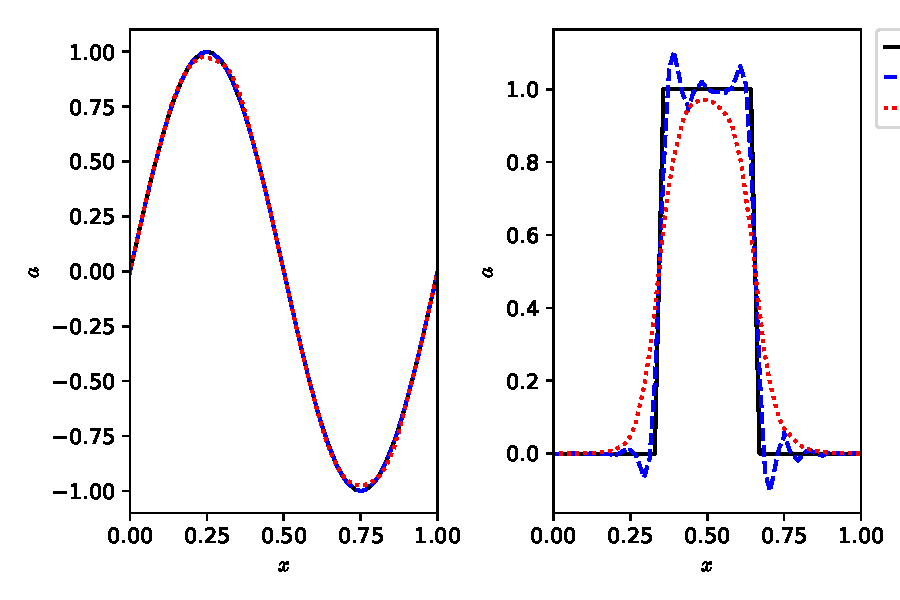
\includegraphics[width=0.8\linewidth]{dg_grid}
\caption[The grid for a Discontinuous Galerkin method]
{\label{fig:dg_grid} The grid for a Discontinuous Galerkin method is split into
cells or elements as indicated by the vertical dashed lines -- here there are
only $4$ cells. Within each cell the solution is represented by an
$m^{\text{th}}$ order polynoial, as shown by the dashed lines. This
representation is central to the modal DG method. Equivalent information can be
stored at specific nodes, as shown by the markers. Note how the number and
location of the nodes varies with $m$. \\
\hydroexdoit{\href{https://github.com/zingale/hydro_examples/blob/master/advection/dg.py}{dg.py}}}
\end{figure}
%
Figure~\ref{fig:dg_grid} shows the nodes and modes for a sine wave represented
by a Discontinuous Galerkin method on a grid with only $4$ cells. We see how
rapidly the representation appears to converge to the smooth sine wave with
increasing $m$. Note also how the locations of the nodes varies with $m$, as the
optimal nodes changes with the order of the method. However, in all cases there
are nodes at the boundaries of each cell.

\begin{exercise}[Vandermonde matrices]
{Construct the Vandermonde matrix converting modal coefficients, based on
orthonormal Legendre polynomials, to nodal coefficients, based on Gauss-Lobatto
nodal points, on the interval $x \in [-1, 1]$. For example, for $m=2$ the result
is, to $4$ significant figures,
%
\begin{equation*}
  V = \begin{pmatrix}
        0.7071 & -1.225 & 1.581 \\
        0.7071 & 0 & -0.7906 \\
        0.7071 & 1.225 & 1.581
      \end{pmatrix}.
\end{equation*}
%
Using the Vandermonde matrix and its inverse, check that you can convert from
nodes to modes and vice versa. Check that the condition number grows slowly with
$m$ (roughly as $m^{1/2}$ for large $m$).}
\end{exercise}

With these restrictions, we can now construct the nodal scheme. As noted above,
this scheme remains a modal scheme as generally introduced in section~\ref{sec:dg_basis},
but the basis functions are the indicator polynomials $\ell_n(x)$. Thus the
scheme can be written in the mass matrix form
%
\begin{equation}
  \tag{\ref{eq:dg_advection5}}
  \hat{M} \ddt{\bm{\hat{a}}} + \hat{S}^T u \bm{\hat{a}} = -\left[ \bm{\psi F} \right]_{-1}^1,
\end{equation}
%
but now the two matrices are given by
%
\begin{align}
  \label{eq:dg_nodal_mass_matrix}
  \hat{M}_{ln} &= \int_{-1}^1 \ell_l(x) \ell_n(x), \\
  \label{eq:dg_nodal_stiffness_matrix}
  \hat{S}_{ln} &= \int_{-1}^1 \ell_l(x) \ddx{\ell_n}(x).
\end{align}
%
By using the Vandermonde matrix to link the nodal basis to an orthogonal basis
such as the Legendre polynomials we can simplify the mass matrix to
%
\begin{equation}
  \label{eq:dg_nodal_mass_matrix_from_V}
  \hat{M} = \left( \hat{V} \hat{V}^T \right)^{-1}.
\end{equation}
%
The stiffness matrix can also be simplified, by re-writing $\ddx{\ell_n}(x)$ as
an expansion in terms of $\ell_n(x)$. Defining the \emph{differentiation matrix}
$\hat{D}$ as
%
\begin{equation}
  \label{eq:dg_nodal_differentiation}
  \hat{D}_{ln} = \left. \ddx{\ell_n}(x) \right|_{x = \xi_l}
\end{equation}
%
we have $\ddx{\ell_n}(x) = \sum_k \hat{D}_{kn} \ell_k(x)$
%
\begin{subequations}
  \label{eq:dg_nodal_stiffness_matrix_from_D_steps}
  \begin{align}
    \hat{S}_{ln} &= \int_{-1}^1 \ell_l(x) \ddx{\ell_n}(x) \\
    &= \int_{-1}^1 \ell_l(x) \sum_k \hat{D}_{kn} \ell_k(x) \\
    &= \sum_k \left( \ell_l(x) \ell_k(x) \right) \hat{D}_{kn} \\
    &= \hat{M}_{lk} \hat{D}_kn.
  \end{align}
\end{subequations}
%
This shows that the stiffness matrix simplifies to
%
\begin{equation}
  \label{eq:dg_nodal_stiffness_matrix_from_V}
  \hat{S} = \hat{M} \hat{D}.
\end{equation}
%
Finally, using similar methods to the steps above, we can link the differentiation
matrix back to the Vandermonde matrix, via
%
\begin{equation}
  \label{eq:dg_nodal_D_matrix_from_V}
  \hat{D} = \left( \ddx{V} \right) \hat{V}^{-1}.
\end{equation}
%
This is primarily useful when the modal function basis is a standard library
function such as the (normalized) Legendre polynomials. This means that the
basis functions and their derivatives, and hence the Vandermonde matrix and its
derivatives, can be written solely in terms of library functions. For example,
in Python the \texttt{numpy} package contains (in \texttt{numpy.polynomial.legendre})
the functions \texttt{legval} (which evaluates the Legendre polynomials),
\texttt{legder} (which links the derivatives of the Legendre polynomials back to
the Legendre polynomials themselves), and \texttt{legvander} (which evaluates
the Vandermonde matrix directly, but in un-normalized form).

There is one final step needed to construct the full scheme. So far, the method
has been built assuming a single element with the coordinates $x \in [-1, 1]$.
For most cases we will want to use a ``small'' number of modes, say $m \le 5$,
and split the domain into $N$ elements, like the cells in a finite volume scheme.
If we assume a general element has coordinates $x \in [x_{j-1/2}, x_{j+1/2}]$
with width $\Delta x$, then the \emph{form} of the scheme remains the same:
%
\begin{equation}
  \label{eq:dg_nodal_final}
  M \ddt{\bm{\hat{a}}} + S^T u \bm{\hat{a}} = -\left[ \bm{\psi F} \right]_{x_{j-1/2}}^{x_{j+1/2}}.
\end{equation}
%
However, the change of coordinates needs to be factored in. We can see how this
works by looking at the integral definitions, such as~\eqref{eq:dg_nodal_mass_matrix}
and~\eqref{eq:dg_nodal_stiffness_matrix}. We see that the mass matrix transforms
as
%
\begin{equation}
  \label{eq:dg_nodal_mass_matrix_with_h}
  M = \frac{\Delta x}{2} \hat{M},
\end{equation}
%
but that the stiffness matrix is unchanged.

\begin{exercise}[Mass and stiffness matrices]
{From the Vandermonde matrices constructed above, build the mass, differentiation
and stiffness matrices $\hat{M}, \hat{D}, \hat{S}$, on the interval
$x \in [-1, 1]$. For example, for $m=2$ the results are, to $4$ significant
figures,
%
\begin{align*}
  \hat{M} &= \begin{pmatrix}
        0.2667 & 0.1333 & -0.0667 \\
        0.1333 & 1.067 & 0.1333 \\
        -0.06667 & 0.1333 & 0.2667
      \end{pmatrix}, \\
  \hat{D} &= \begin{pmatrix}
        -1.5 & 2 & -0.5 \\
        -0.5 & 0 & 0.5 \\
        0.5 & -2 & 1.5
      \end{pmatrix}, \\
  \hat{S} &= \begin{pmatrix}
        -0.5 & 0.6667 & -1.667 \\
        -0.6667 & 0 & 0.6667 \\
        1.667 & -0.6667 & 0.5
      \end{pmatrix}.
\end{align*}
}
\end{exercise}

\begin{figure}[t]
\centering
% figure generated by hydro_examples/advection/dg.py
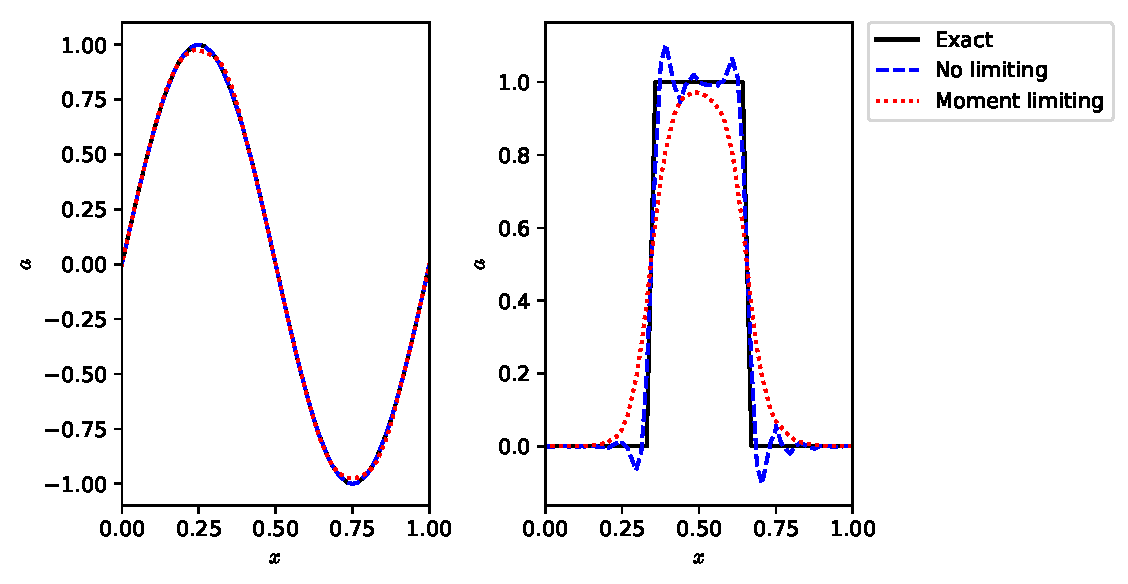
\includegraphics[width=0.8\linewidth]{dg_limiter}
\caption[Discontinuous Galerkin methods in action]
{\label{fig:dg_limiter} The left panel shows a Discontinuous Galerkin method
with $m=3$ and $16$ elements applied to the advection equation, where a sine
wave is advected once around the domain. Even at this low resolution the result
without limiting is visually exact, and using moment limiting is very accurate.
In the right panel the same methods are applied to the ``top hat'' initial data,
again advected once the periodic domain. The unlimited method shows the expected
Gibbs oscillations, which are confined to the elements next to the
discontinuities. The moment limited method shows no oscillations. \\
\hydroexdoit{\href{https://github.com/zingale/hydro_examples/blob/master/advection/dg.py}{dg.py}}}
\end{figure}
%
By combining the nodal DG update described above with a time integrator we can
look at the performance of the scheme. We need to take care in choosing the
timestep. From the nodal point of view we can see that the width of the cell,
$\Delta x$, is not going to be the limiting factor. Instead, the smallest
distance between the (unequally spaced!) nodes is going to be crucial. General
results (see e.g.~\cite{hesthaven2018numerical}) suggest that reducing the
timestep by a factor of $2 m + 1$ is sufficient to ensure stability, but it does
increase computational cost.

Figure~\ref{fig:dg_limiter} advects two initial profiles one period around a
periodic domain. In the left panel we see the excellent performance when applied
to a smooth profile. The unlimited method is essentially indistinguishable from
the exact solution. However, the right panel shows that when the unlimited
method is applied to a discontinuous initial profile then Gibbs oscillations
result. The only ``nice'' feature of the Discontinuous Galerkin method here is
that these oscillations are confined to the elements next to the
discontinuities, and do not spread to cover the entire grid.

As with finite difference schemes, there are a range of modifications that can
be made to limit or eliminate these oscillations. In Discontinuous Galerkin
methods it is typical to do this in two steps: first, identify which elements
need limiting, and second, modify the data in the required cells. The
identification step can be done using the nodal values: construct limited slopes
from cell average values and compare the predicted values at cell boundaries to
the nodal values actually stored. The modification step can be done in many
ways. A number are outlined in~\cite{hesthaven2018numerical}, but here we show a
method that modifies the modal values, rather than the nodal values, as
developed by~\cite{burbeau2001problem}. This \emph{moment limiting} approach
removes the oscillations, as seen in Figure~\ref{fig:dg_limiter}.

\begin{figure}[t]
\centering
% figure generated by hydro_examples/advection/dg.py
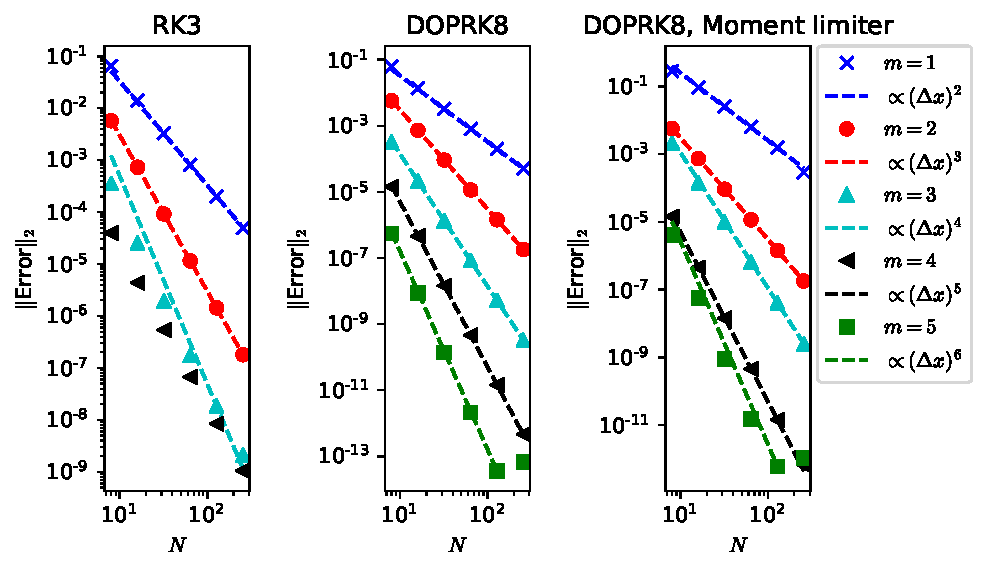
\includegraphics[width=0.8\linewidth]{dg_convergence_sine}
\caption[Convergence of Discontinuous Galerkin methods]
{\label{fig:dg_convergence_sine} Each panel shows the convergence of the
Discontinuous Galerkin methods for $m = 1, \dots, 5$, when using different time
integrators (the left panel uses RK3, the other panels an $8^{\text{th}}$ order
RK method) or using limiters (the right panel uses moment limiting, whilst the
other panels use no limiting). The expected convergence rate should be $m+1$,
which is seen only for the low order methods when the time integrator is RK3.
For higher $m$ schemes the error from the time integrator dominates, but using
a higher order time integrator shows that the expected convergence rate can be
recovered, as seen in the central and right panel. Comparing the central and
right panel we see that it is possible, with moment limiting, to retain the high
order convergence, but that moment limiting increase the absolute error by
roughly an order of magnitude. \\
\hydroexdoit{\href{https://github.com/zingale/hydro_examples/blob/master/advection/dg.py}{dg.py}}}
\end{figure}
%
The Discontinuous Galerkin methods are constructed to have high-order accuracy.
In principle, the convergence rate should be $\propto (\Delta x)^{m+1}$. As with
the WENO schemes above this can be difficult to see in reality.
Figure~\ref{fig:dg_convergence_sine} shows the convergence rate when advecting
a sine wave once around a periodic domain. In the left panel the third order
SSP RK3 time integrator has been used. The expected $2^{\text{nd}}$ and
$3^{\text{rd}}$ order convergence is seen for $m=1$ and $m=2$. However, for
higher orders the limitations of the third-order time integrator reduce the
convergence rate.

In the central panel of Figure~\ref{fig:dg_convergence_sine} an $8^{\text{th}}$
order time integrator is used. This reduces the time integrator error far below
what is needed, and we now see that every scheme converges at the expected rate.
In more complex systems in multiple dimensions the error from the spatial terms
will be much larger, and so the RK3 method can be used without compromising the
accuracy. The right panel shows that the moment limiter does not affect the
convergence rate of the method, although it does increase the absolute error in
nearly all cases.

\begin{figure}[t]
\centering
% figure generated by hydro_examples/advection/compare_schemes.py
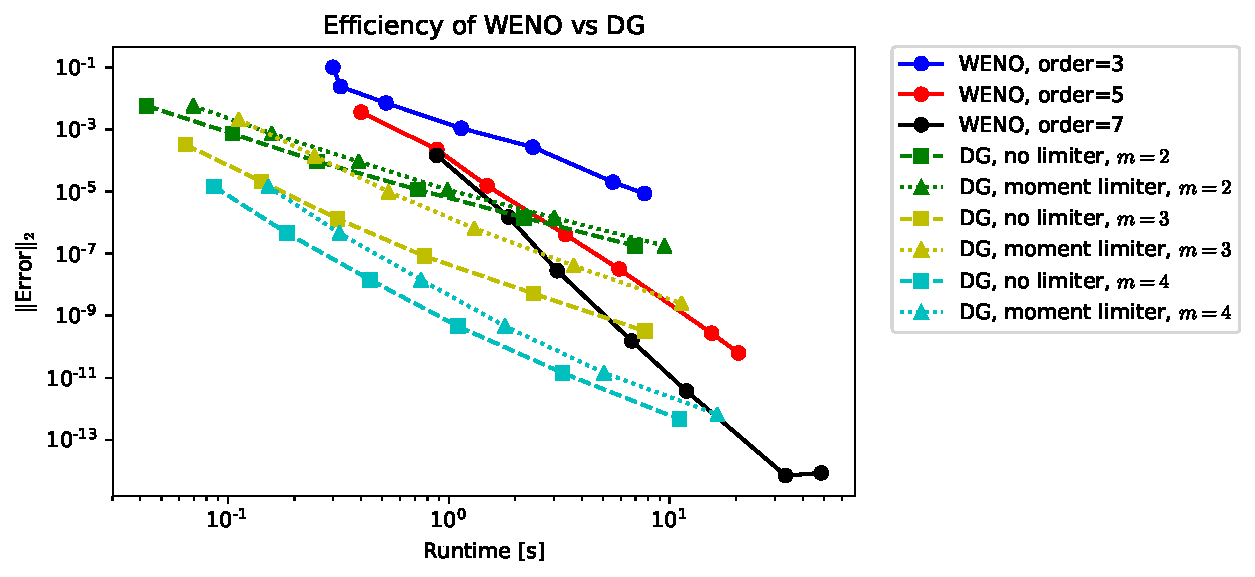
\includegraphics[width=0.8\linewidth]{dg_weno_efficiency}
\caption[Efficiency of high order methods]
{\label{fig:dg_weno_efficiency} Comparing a Discontinuous Galerkin scheme to a
finite difference or finite volume scheme needs some care, as the number of
cells used stops being a fair comparison: the DG method stores $m+1$ times more
information per cell than a typical finite difference scheme. Instead, it is
better to compare the efficiency of the methods -- for example, by comparing
the runtime required to get a solution with a certain accuracy. This figure
shows the efficiency for high order DG and WENO schemes, by advecting a sine
wave once around a periodic domain and comparing the errors. By comparing the
plain Python WENO implementation to one optimized using \texttt{numba} we see
the importance of the specific implementation. The impact of higher order
schemes is also apparent.\\
\hydroexdoit{\href{https://github.com/zingale/hydro_examples/blob/master/advection/compare_schemes.py}{compare\_schemes.py}}}
\end{figure}
%
When comparing the errors produced by a second order scheme (as shown in
Figure~\ref{fig:advnorm}) or a WENO scheme (as shown in
Figure~\ref{fig:weno-converge-sine}) with those produced by a Discontinuous
Galerkin scheme (as shown in Figure~\ref{fig:dg_convergence_sine}), we need to
be careful to interpret the results fairly. Leave aside that the results for the
second order schemes come from advecting different profiles for longer times.
More importantly we should note that Discontinuous Galerkin schemes use far more
resources for each cell: $m+1$ nodes of information are stored per cell, rather
than the single value used for a finite volume or finite difference scheme.

Instead it is better to compare the efficiency of the method, by measuring how
long it takes, and how much resources (e.g., memory) it requires, to reach a
certain accuracy. This can be very implementation specific, so should also be
done carefully. An example of this, comparing WENO and DG schemes, is given in
Figure~\ref{fig:dg_weno_efficiency}. We see that higher-order schemes increase
in efficiency with more resources, as expected (the WENO7 scheme converges at
$13^{\text{th}}$ order, compared to the DG4 scheme which converges at
$5^{\text{th}}$ order). However, for this problem where the data remains very
smooth, the Discontinuous Galerkin methods are clearly better, even with
limiting on. The importance of the specific implementation is also shown by
comparing to an optimized WENO code using the just-in-time \texttt{numba}
module. The structure of the DG code makes it harder to optimize. The advantage
that the DG code has over the plain Python WENO implementation may also depend
on the initial data, and may not remain when discontinuities appear.

\section{Going further}

\begin{itemize}

\item {\em Slope limiting}: there are a wide variety of slope
  limiters.  All of them are designed to reduce oscillations in the
  presence of discontinuities or extrema, but some are higher-order
  and can be less restrictive when dealing with smooth flows.  Most
  hydro texts (e.g.\ \cite{leveque:2002,toro:1997}) provide an
  introduction to the design of such limiters.

\item {\em Multi-dimensional limiting}: the procedure described above
  still does the limiting in each dimension independent of the other
  when doing the unsplit reconstruction.  This can lead to overshoots/
  undershoots.  An example of a method that considers the limiting
  in multi-dimensions is \cite{BDS,quadBDS}.

\item {\em Spatially-varying velocity field}: if we consider a spatially
  varying velocity field, $u(x,y)$ and $v(x,y)$ that is specified externally,
  then we can describe the advection of a quantity $\phi$ as:
  \begin{equation}
  \phi_t + (\phi u)_x + (\phi v)_y = 0
  \end{equation}
  The solution procedure is largely the same as described above.  We write:
\begin{align}
\phi_{i+\myhalf,j,L}^{n+\myhalf} &= \phi_{i,j}^n +
   \frac{\Delta x}{2} \frac{\partial \phi}{\partial x} +
   \frac{\Delta t}{2} \frac{\partial \phi}{\partial t} + \ldots \nonumber \\
%
 &= \phi_{i,j}^n +
    \frac{\Delta x}{2} \frac{\partial \phi}{\partial x} +
    \frac{\Delta t}{2} \left [ -(\phi u)_x -(\phi v)_y \right ]_{i,j} \nonumber\\
%
 &= \underbrace{\phi_{i,j}^n +
   \frac{\Delta x}{2} \left ( 1 - \frac{\Delta t}{\Delta x} u_{i,j} \right )
        \frac{\partial \phi}{\partial x}}_{\hat{\phi}_{i+\myhalf,j,L}^{n+\myhalf}}
   - \frac{\Delta t}{2} \left [\phi u_x \right ]_{i,j}
   - \frac{\Delta t}{2} \left [ (\phi v)_y \right ]_{i,j}
\end{align}
  and upwinding is used to resolve the Riemann problem for both the
  transverse and normal interface states.  This type of construction
  comes up in low Mach number flows, where the density can be advected
  according to the velocity field in much the fashion shown here, and
  is described in \S~\ref{sec:lm:density}.


  For compressible hydrodynamics, we often have density-weighted quantities
  that we advect.  This extension is described in \S~\ref{sec:euler:further}.

\end{itemize}


\section{\pyro\ experimentation}

To gain some experiences with these ideas, we can use the advection
solver in \pyro\ (see Appendix~\ref{app:pyro} to get started).
The \pyro\ advection solver implements the second-order unsplit
advection algorithm described in the previous sections.  To run
this solver on the Gaussian advection problem, do:
\begin{verbatim}
./pyro.py advection smooth inputs.smooth
\end{verbatim}
By default, this will advect a Gaussian profile diagonally across the
domain for a single period.

To get a feel for the advection algorithm, here are some suggested
exercises:

\begin{exercise}[Role of limiters]
{Implement a tophat initial profile and run with and without limiters
  (this is controlled by the {\tt advection.limiter} runtime
  parameter).}
\end{exercise}

\begin{exercise}[Grid effects]
{Look at the solution when you advect purely in the $x$- or
  $y$-direction and compare to the diagonal case---notice how the
  direction affects the error in the solution.  This is the imprint
  of the grid we discretize on.}
\end{exercise}

\begin{exercise}[Split vs.\ unsplit]
{Implement a dimensionally-split version of the advection algorithm
and compare the results to the unsplit version.  Pick a suitable norm
and measure the convergence of the methods.}
\end{exercise}
